% !TeX root = ../main.tex
% =========================================================================
% CAPÍTULO 1. INTRODUCCIÓN Y ANÁLISIS
% =========================================================================

\capitulopage{Capítulo I}

\setcounter{section}{1}
\setcounter{subsection}{0}

\addcontentsline{toc}{section}{Capítulo 1. Introducción y Análisis}

\begin{center}
    {\normalfont\Large\bfseries I. Introducción y Análisis \par}
\end{center}
% -------------------------------------------------------------------------
% 1.1. INTRODUCCIÓN
% -------------------------------------------------------------------------
\subsection{Introducción}
La ingeniería de software moderna depende en gran medida de la reutilización intensiva de paquetes y librerías de código abierto, conformando hasta el 80\% de la base de código ejecutable dentro del ecosistema de desarrollo en Python y en los flujos de integración continua (CI/CD) \parencite{synopsys2024ossra, decan2019empirical}. %[cite: 5]
Sin embargo, este paradigma expone a las organizaciones a fallos estructurales en la cadena de suministro de software (\textit{software supply chain}), donde los componentes de terceros introducen vulnerabilidades y exposiciones comunes (CVE) que comprometen la integridad de las aplicaciones \parencite{ladisa2023sok, owasp2025top10}. %[cite: 5]

El presente Proyecto de Fin de Carrera se sitúa y valida en el entorno operacional de \textbf{Lidercom Perú S.A.C.}, empresa de tecnología educativa (\textit{EdTech}) orientada a la medición y entrenamiento de competencias socioemocionales y de liderazgo mediante analítica de datos y procesamiento de lenguaje natural (NLP) en Python. %[cite: 4]
Debido a la naturaleza confidencial de la información gestionada y la propiedad intelectual de sus modelos predictivos, la organización exige garantizar la seguridad de su software bajo la norma internacional \textbf{ISO/IEC 27001:2022} (Controles A.8.8, A.8.12 y A.8.28), lo que prohíbe taxativamente el uso de plataformas comerciales SaaS que extraen código fuente o metadatos hacia servidores en la nube \parencite{gutierrez2024auditoria, ladisa2023sok}. %[cite: 3, 4]

Frente a esta necesidad, el propósito general del proyecto es diseñar e implementar \textbf{\textit{PyReach}}, un analizador estático en línea de comandos (CLI) de ejecución 100\% local (\textit{on-premise}) para Python 3.10+ que construye Grafos de Llamadas (\textit{Call Graphs}) interprocedimentales analizando el Árbol de Sintaxis Abstracta (AST) del código fuente y sus dependencias en \texttt{site-packages} \parencite{salis2021pycg, ryder1979constructing}. %[cite: 2, 4, 5]
\textit{PyReach} determina formalmente si las funciones afectadas por CVEs reportadas en OpenSSF OSV son alcanzables en ejecución, descartando alertas espurias en el pipeline de CI/CD sin comprometer la privacidad del código corporativo \parencite{openssf2023osv, oasis2019sarif, humble2010continuous}. %[cite: 3, 5]

El presente capítulo sigue la estructura metodológica de la Unidad 1 del libro de cátedra \parencite{torres2026proyecto} %[cite: 7]
y se organiza formalmente en las siguientes secciones: el planteamiento y formulación del problema junto con el árbol de problemas (1.2); %[cite: 1]
la descripción del proyecto, sus objetivos y matriz de trazabilidad (1.3); %[cite: 1]
la justificación técnica y económica (1.4); %[cite: 1]
la delimitación del alcance, exclusiones, limitaciones y protección de datos (1.5); %[cite: 1]
el diseño metodológico cuantitativo (1.6); %[cite: 1]
la identificación y categorización de stakeholders (1.7); %[cite: 1]
el análisis de antecedentes (1.8) y estado del arte (1.9); %[cite: 1]
la declaración de estándares y herramientas (1.10); %[cite: 1]
la especificación formal de requerimientos y casos de uso (1.11); %[cite: 1]
el análisis multicriterio de alternativas (1.12); %[cite: 1]
la evaluación de brechas, beneficios y viabilidad financiera (1.13); %[cite: 1]
el balance de trade-offs ante la triple restricción (1.14); %[cite: 1]
y la planificación integral de cronograma, costos paramétricos y riesgos del proyecto (1.15) \parencite{pmi2021pmbok, wiegers2013software, torres2026proyecto}. %[cite: 1, 7]

% -------------------------------------------------------------------------
% 1.2. PLANTEAMIENTO Y FORMULACIÓN DEL PROBLEMA
% -------------------------------------------------------------------------
\subsection{Planteamiento y Formulación del Problema}

\subsubsection{Planteamiento del Problema}
En el desarrollo ágil de software bajo el paradigma DevSecOps, la incorporación de escáneres automáticos de Análisis de Composición de Software (SCA) busca prevenir brechas de seguridad de forma temprana en los pipelines de CI/CD \parencite{humble2010continuous, coila2023devsecops}. %[cite: 3]
No obstante, las herramientas SCA tradicionales operan a nivel superficial inspeccionando únicamente archivos de manifiesto (\texttt{requirements.txt}, \texttt{poetry.lock}, \texttt{uv.lock}), asumiendo erróneamente que la sola presencia de una librería en disco equivale a la ejecución efectiva de su código vulnerable \parencite{pashchenko2022vuln4real, dann2021identifying}. %[cite: 4, 5]

Dado que las aplicaciones suelen invocar únicamente subconjuntos reducidos de sus dependencias, más del 80\% al 90\% de las alertas emitidas por escáneres basados en manifiestos corresponden a funciones y métodos inalcanzables (código muerto respecto al vector de ataque) \parencite{pashchenko2022vuln4real, ponta2020detection}. %[cite: 4, 5]
En el contexto real de \textbf{Lidercom Perú S.A.C.}, los desarrolladores de microservicios de analítica y NLP en Python reciben semanalmente decenas de alertas bloqueantes sobre librerías transitivas. %[cite: 4, 5]
Al no discriminar la herramienta si el código vulnerable es realmente invocado, dos ingenieros de software de la empresa deben destinar conjuntamente un promedio de 10 horas semanales a revisar y descartar manualmente alertas no explotables \parencite{sadowski2018lessons}. %[cite: 2]

Esta sobrecarga operativa produce tres efectos adversos directos: fatiga de alertas (\textit{alert fatigue}) en los desarrolladores que induce a la desatención de vulnerabilidades críticas reales \parencite{johnson2013developers}; %[cite: 4, 5]
retrasos en los despliegues de CI/CD por actualizaciones forzadas de dependencias que introducen incompatibilidades de API (\textit{breaking changes}) \parencite{bogart2016break, fowler2018refactoring}; %[cite: 4, 5]
y un sobrecosto acumulado en horas de ingeniería que no puede resolverse mediante plataformas comerciales SaaS sin vulnerar la soberanía del código fuente exigida por la norma ISO/IEC 27001:2022 \parencite{ladisa2023sok, gutierrez2024auditoria}. %[cite: 4, 5]

\newpage

\subsubsection{Árbol de Problemas}
En la Figura \ref{fig:arbol_problemas} se ilustra visualmente la estructura causal de causas y efectos desarrollada para el proyecto. %[cite: 5]
Asimismo, en la Tabla \ref{tab:arbol_problemas_tabla} se detalla su matriz analítica siguiendo la metodología del marco lógico y los lineamientos de la Unidad 2 del libro de cátedra \parencite{ torres2026proyecto}.

\begin{figure}[H]
\centering
\includegraphics[width=0.88\textwidth]{../figuras/figuras1/mermaid-diagram-2026-08-17-222626.png}
\caption{Árbol de problemas: causas, problema central y efectos en la remediación de dependencias transitivas}
\label{fig:arbol_problemas}
\end{figure}

\begin{table}[H]
\centering
\caption{Árbol de problemas del proyecto}
\label{tab:arbol_problemas_tabla}
\small
\setstretch{1.10}
\begin{tabularx}{\textwidth}{>{\bfseries\raggedright\arraybackslash}p{4.0cm} X}
\toprule
\textbf{Nivel} & \textbf{Elemento} \\
\midrule
Planteamiento & Elevada e incontrolada tasa de alertas de vulnerabilidad irrelevantes generadas sobre dependencias transitivas no ejecutadas en los microservicios Python de analítica y NLP en Lidercom Perú S.A.C. \\
\addlinespace
Efecto & Fatiga de alertas en desarrolladores y desatención de vulnerabilidades que sí representan riesgo crítico real \parencite{sadowski2018lessons, johnson2013developers}. \\
\addlinespace
Efecto & Retrasos en pipelines CI/CD y fallos en producción por actualizaciones innecesarias de librerías \parencite{bogart2016break, humble2010continuous}. \\
\addlinespace
Efecto & Sobrecosto en horas de ingeniería dedicadas a clasificar manualmente falsas alarmas de seguridad en microservicios \parencite{pashchenko2022vuln4real}. \\
\midrule
Problema central & \textbf{Ineficiencia en la priorización y mitigación de vulnerabilidades en la cadena de suministro de software por alta tasa de alertas no explotables en dependencias transitivas.} \\
\midrule
Causa directa & Herramientas SCA limitadas a inspección superficial basada exclusivamente en comparación de versiones en manifiestos \parencite{vargas2022analisis}. \\
\addlinespace
Causa directa & Carencia de Call Graphs que resuelvan cadenas transitivas profundas y analicen paquetes anidados en \texttt{site-packages} \parencite{salis2021pycg, alfadel2023empirical}. \\
\addlinespace
Causa raíz & Dependencia de suites SaaS propietarias con bases de datos cerradas y sin reachability local, contraviniendo ISO/IEC 27001 \parencite{ladisa2023sok, gutierrez2024auditoria}. \\
\bottomrule
\end{tabularx}
\end{table}

\subsubsection{Formulación del Problema}
En concordancia con el problema central del árbol causal y las pautas metodológicas de la Unidad 2 \parencite{torres2026proyecto}, se define la formulación del problema como la siguiente pregunta general de investigación: %[cite: 1, 7]

\vspace{0.3cm}
\noindent
\textbf{¿De qué manera un analizador estático de código basado en grafos de llamadas (\textit{reachability analysis}) para dependencias transitivas en Python permite reducir la tasa de alertas de vulnerabilidad no explotables generadas en el ciclo de vida del software en Lidercom Perú S.A.C.?}

% -------------------------------------------------------------------------
% 1.3. DESCRIPCIÓN DEL PROYECTO
% -------------------------------------------------------------------------
\subsection{Descripción del Proyecto}
La descripción técnica del proyecto delimita la intervención de ingeniería sobre el proceso de gestión de vulnerabilidades en \textbf{Lidercom Perú S.A.C.}, traduciendo las causas principales del problema en metas medibles y verificables mediante un artefacto de software.
El propósito central es dotar a la organización de un mecanismo formal de análisis estático interprocedimental que permita discernir si las librerías transitivas vulnerables son efectivamente ejecutadas por sus microservicios, optimizando el triaje de seguridad sin vulnerar la soberanía del código fuente bajo la norma ISO/IEC 27001:2022 \parencite{ladisa2023sok, gutierrez2024auditoria}. %[cite: 4, 5]

\subsubsection{Objetivo General}
En estricta correspondencia con la formulación del problema y cumpliendo con la directriz metodológica de presentar un único verbo rector en infinitivo y un solo propósito cardinal \parencite{torres2026proyecto}, se define el objetivo general del proyecto: %[cite: 1, 7]

\vspace{0.2cm}
\noindent
\textbf{Implementar un analizador estático de alcanzabilidad interprocedimental sobre el Árbol de Sintaxis Abstracta (AST) para proyectos en lenguaje Python, que reduzca la tasa de alertas de vulnerabilidad no explotables en dependencias transitivas y optimice la priorización de seguridad en el pipeline de desarrollo de Lidercom Perú S.A.C.} %[cite: 1, 5]

\subsubsection{Objetivos Específicos}
El objetivo general se descompone jerárquicamente en cuatro objetivos específicos medibles, orientados a resultados y correspondientes a los hitos de entrega del ciclo de vida del proyecto \parencite{torres2026proyecto, pmi2021pmbok}: %[cite: 1, 7]

\begin{enumerate}[leftmargin=1.27cm, label=\textbf{OE\arabic*.}]
    \item \textbf{Analizar y extraer} metadatos estructurados de vulnerabilidades y funciones afectadas a partir del esquema abierto OpenSSF OSV para el ecosistema PyPI, habilitando un catálogo local indexado en SQLite para consultas fuera de línea (\textit{offline}) \parencite{openssf2023osv}. %[cite: 3, 5]
    \item \textbf{Diseñar} el modelo arquitectónico y el algoritmo de construcción de Grafos de Llamadas (\textit{Call Graphs}) interprocedimentales a partir del recorrido del Árbol de Sintaxis Abstracta (AST) en Python 3.10+, abarcando código de la aplicación huésped y dependencias anidadas en \texttt{site-packages} \parencite{salis2021pycg, ryder1979constructing}. %[cite: 2, 4, 5]
    \item \textbf{Construir} la herramienta ejecutable en línea de comandos (CLI) denominada \textit{PyReach}, que determine la existencia de caminos dirigidos entre los puntos de entrada (\textit{entrypoints}) y los nodos vulnerables, clasificando las alertas y exportando diagnósticos en el estándar formal OASIS SARIF v2.1.0 para compuertas de calidad en integración continua \parencite{oasis2019sarif, humble2010continuous}. %[cite: 3, 5]
    \item \textbf{Validar} cuantitativamente la tasa de reducción de falsos positivos ($\ge 70\%$) y la eficiencia temporal en pipelines locales frente a escáneres SCA tradicionales basados en manifiestos, mediante pruebas experimentales sobre el corpus real de microservicios de analítica y NLP de Lidercom Perú S.A.C. \parencite{pashchenko2022vuln4real, wohlin2012experimentation}. %[cite: 3, 4, 5]
\end{enumerate}

En la Figura \ref{fig:arbol_objetivos} se esquematiza el árbol de objetivos que articula la relación directa entre el objetivo general y sus productos específicos.

\begin{figure}[H]
\centering
\includegraphics[width=0.88\textwidth]{../figuras/figuras1/mermaid-diagram-2026-08-17-222720.png}
\caption{Árbol de objetivos: del objetivo general a los específicos}
\label{fig:arbol_objetivos}
\end{figure}

\subsubsection{Matriz Objetivo--Resultado--Capítulo}
Siguiendo las directrices de la Unidad 3 del libro de cátedra \parencite{torres2026proyecto}, en la Tabla \ref{tab:matriz_obj_res} se establece la matriz de trazabilidad que vincula cada objetivo específico con su entregable tangible y el capítulo formal donde se demuestra su cumplimiento. %[cite: 1, 7]

\begin{table}[H]
\centering
\caption{Matriz objetivo--resultado--capítulo}
\label{tab:matriz_obj_res}
\small
\setstretch{1.10}
\begin{tabularx}{\textwidth}{>{\raggedright\arraybackslash}p{4.8cm} >{\raggedright\arraybackslash}X >{\centering\arraybackslash}p{3.8cm}}
\toprule
\textbf{Objetivo específico} & \textbf{Resultado esperado} & \textbf{Capítulo donde se sustenta} \\
\midrule
OE1. Analizar y extraer metadatos de vulnerabilidades desde OSV.dev a nivel de función/símbolo específico. & 
Módulo de ingesta (\texttt{pyreach-ingest}) y base de datos local SQLite con advisories indexados por paquete, versión y función vulnerable. & 
Capítulo 1 (Introducción y Análisis) / Capítulo 2. \\ 
\addlinespace
OE2. Diseñar el algoritmo de grafos de llamadas inter-módulo a partir del AST de Python. & 
Especificación algorítmica formal, diseño arquitectónico en capas y modelo de grafos dirigidos interprocedimentales (\textit{Call Graph}). & 
Capítulo 2 (Desarrollo del Proyecto). \\ 
\addlinespace
OE3. Construir la herramienta CLI con salida en formato SARIF/JSON e integración a CI/CD. & 
Artefacto ejecutable CLI \textit{PyReach}, serializador bajo esquema OASIS SARIF v2.1.0 y compuertas de calidad integrables a runners locales. & 
Capítulo 2 (Desarrollo del Proyecto). \\ 
\addlinespace
OE4. Validar la tasa de reducción de alertas y precisión frente a herramientas estándar. & 
Informe experimental con matrices de confusión, curvas de precisión/recall, reducción porcentual de alertas ($\ge 70\%$) y tiempos de ejecución. & 
Capítulo 3 (Validación y Presentación). \\ 
\bottomrule
\end{tabularx}
\end{table}

% -------------------------------------------------------------------------
% 1.4. JUSTIFICACIÓN DEL PROYECTO
% -------------------------------------------------------------------------
\subsection{Justificación del Proyecto}
La justificación sustenta el valor técnico y organizacional que fundamenta el desarrollo de la solución \parencite{sommerville2016software, pressman2020software}. En el ámbito técnico, las herramientas convencionales de Análisis de Composición de Software (SCA) realizan una equiparación estática superficial de cadenas de texto en manifiestos, asumiendo una sobreestimación que genera más del 80\% de alertas falsas en dependencias transitivas no ejecutadas \parencite{pashchenko2022vuln4real, dann2021identifying}. %[cite: 4, 5]
Las soluciones comerciales con soporte de alcanzabilidad (\textit{reachability analysis}) operan bajo esquemas cerrados en la nube que vulneran la privacidad del código fuente \parencite{endorlabs2023state, ladisa2023sok}. %[cite: 4]
Diseñar un generador de Grafos de Llamadas sobre el AST nativo de Python 3.10+ capaz de recorrer \texttt{site-packages} permite discriminar formalmente si una función con CVE posee una ruta de control activa desde los puntos de entrada (\textit{entrypoints}) de la aplicación \parencite{salis2021pycg, ryder1979constructing}, garantizando la soberanía del código ($0\text{ bytes}$ en nube) conforme al Control A.8.12 de ISO/IEC 27001:2022 \parencite{gutierrez2024auditoria}. %[cite: 2, 4, 5]

En el ámbito económico y organizacional, los equipos ágiles de ingeniería destinan entre un 20\% y un 30\% de su jornada al triaje manual de alertas de seguridad irrelevantes \parencite{johnson2013developers, sadowski2018lessons}. %[cite: 4, 5]
En Lidercom Perú S.A.C., filtrar automáticamente al menos el 70\% de estas alertas espurias recupera 28 horas-hombre de ingeniería al mes, lo que representa un beneficio económico directo de S/ 8,400.00 anuales \parencite{torres2026proyecto}. %[cite: 2]
Asimismo, se evita el gasto recurrente de licencias comerciales extranjeras (cotizadas entre \$60 y \$120 USD mensuales por desarrollador), protegiendo la estabilidad del flujo continuo de entregas (\textit{Continuous Delivery}) y reduciendo incidentes en producción causados por actualizaciones innecesarias que introducen roturas de compatibilidad (\textit{breaking changes}) \parencite{bogart2016break, humble2010continuous}. %[cite: 2, 4, 5]

En la Tabla \ref{tab:justificacion} se consolida la justificación técnica y económica del proyecto según el formato de la Unidad 4 del libro de cátedra \parencite{torres2026proyecto}. %[cite: 1, 7]

\begin{table}[H]
\centering
\caption{Justificación técnica y económica del proyecto}
\label{tab:justificacion}
\small
\setstretch{1.10}
\begin{tabularx}{\textwidth}{>{\bfseries\raggedright\arraybackslash}p{4.2cm} X}
\toprule
\textbf{Tipo de justificación} & \textbf{Contenido} \\
\midrule
Técnica & 
Los escáneres SCA convencionales omiten las rutas de invocación del código en reposo. Implementar un generador de Grafos de Llamadas (\textit{Call Graphs}) interprocedimentales sobre el AST nativo de Python permite verificar formalmente si una función vulnerable es alcanzable desde la aplicación, dotando de interpretabilidad al diagnóstico, reduciendo falsos positivos ($\ge 70\%$) y garantizando la soberanía de código ($0\text{ bytes}$ en nube, Control A.8.12 ISO/IEC 27001:2022) sin depender de servicios SaaS externos \parencite{salis2021pycg, ladisa2023sok, gutierrez2024auditoria}. \\ %[cite: 3, 4, 5]
\addlinespace
Organizacional / económica & 
El triaje manual de falsas alertas consume horas críticas de ingeniería. Reducir el 70\% de alertas espurias en Lidercom Perú S.A.C. recupera 28 HH mensuales (S/ 8,400.00 anuales), elimina costos recurrentes de licenciamiento SaaS privativo en dólares (\$1,440.00 USD anuales por 2 asientos), previene fallos operativos derivados de actualizaciones forzadas de librerías (\textit{breaking changes}) y mitiga el riesgo de abandono de compuertas de calidad por fatiga de alertas \parencite{pashchenko2022vuln4real, bogart2016break, sadowski2018lessons}. \\ %[cite: 2, 4, 5]
\bottomrule
\end{tabularx}
\end{table}

% -------------------------------------------------------------------------
% 1.5. ALCANCES Y LIMITACIONES
% -------------------------------------------------------------------------
\subsection{Alcances y Limitaciones}

\subsubsection{Delimitación de Alcance}
La delimitación del alcance define de manera cerrada las fronteras del software, declarando explícitamente los módulos y procesos cubiertos para evitar ambigüedades operativas \parencite{wiegers2013software, torres2026proyecto}. %[cite: 1, 7]
En la Figura \ref{fig:delimitacion_alcance} se esquematiza la demarcación visual de los componentes dentro y fuera del alcance del analizador \textit{PyReach}. %[cite: 5]

\begin{figure}[H]
\centering
\includegraphics[width=0.88\textwidth]{../figuras/figuras1/mermaid-diagram-2026-08-17-222822.png}
\caption{Delimitación del alcance: módulos incluidos y excluidos}
\label{fig:delimitacion_alcance}
\end{figure}

En la Tabla \ref{tab:delimitacion_modulos} se formaliza la delimitación módulo por módulo, detallando el estado de inclusión o exclusión y su respectiva justificación técnica. %[cite: 1, 7]

\begin{table}[H]
\centering
\caption{Delimitación de alcance}
\label{tab:delimitacion_modulos}
\small
\setstretch{1.10}
\begin{tabularx}{\textwidth}{>{\raggedright\arraybackslash}p{4.8cm} >{\centering\arraybackslash}p{3.2cm} >{\raggedright\arraybackslash}X}
\toprule
\textbf{Módulo o proceso} & \textbf{Incluido / Excluido} & \textbf{Justificación} \\
\midrule
Ingesta de manifiestos y consumo de API OSV.dev & Incluido & 
Permite extraer dependencias directas y transitivas (\texttt{requirements.txt}, \texttt{poetry.lock}, \texttt{uv.lock}) e indexar funciones vulnerables de acceso abierto \parencite{openssf2023osv}. \\ %[cite: 5]
\addlinespace
Integración con bases comerciales de pago (Snyk, Veracode) & Excluido & 
El sistema se sustenta 100\% en bases abiertas y reproducibles, evitando costos de suscripción y dependencias propietarias \parencite{torres2026proyecto}. \\ %[cite: 5, 7]
\addlinespace
Constructor de AST y Grafo de Llamadas inter-módulo & Incluido & 
Constituye el núcleo técnico para inspeccionar la sintaxis y enlazar llamadas interprocedimentales hacia paquetes en \texttt{site-packages} \parencite{salis2021pycg}. \\ %[cite: 5]
\addlinespace
Análisis de binarios y extensiones C/C++ (NumPy, Cython) & Excluido & 
Escapa de la ventana temporal del curso; el análisis rastrea código Python interpretado hasta la frontera de invocación externa \parencite{salis2021pycg, torres2026proyecto}. \\ %[cite: 4, 5, 7]
\addlinespace
Motor de alcanzabilidad y búsqueda de rutas dirigidas & Incluido & 
Determina la existencia de caminos dirigidos entre los \textit{entrypoints} de la aplicación y las funciones con CVE para clasificar el estado de la alerta \parencite{ryder1979constructing}. \\ %[cite: 5]
\addlinespace
Generador de reportes CLI y serializador OASIS SARIF v2.1.0 & Incluido & 
Habilita la visualización formateada en consola y la interoperabilidad nativa con pestañas de seguridad en GitHub Actions y GitLab CI \parencite{oasis2019sarif}. \\ %[cite: 5]
\addlinespace
Auto-remediación o parchado automático de código fuente & Excluido & 
El propósito del analizador es de diagnóstico, clasificación y priorización de riesgos, no de refactorización o edición del código fuente \parencite{bogart2016break}. \\ %[cite: 5]
\addlinespace
Análisis dinámico en tiempo de ejecución (DAST / Fuzzing) & Excluido & 
El artefacto se restringe al paradigma de análisis estático (SAST) sobre código en reposo, garantizando tiempos de ejecución reducidos en CI/CD \parencite{humble2010continuous}. \\ %[cite: 5]
\bottomrule
\end{tabularx}
\end{table}

\subsubsection{Limitaciones}
Las limitaciones reconocen de forma explícita las restricciones metodológicas, técnicas y de recursos que condicionan el desarrollo del proyecto \parencite{sommerville2016software, torres2026proyecto}: %[cite: 1, 7]
\begin{itemize}[leftmargin=1.27cm]
    \item \textbf{Restricción de versiones del lenguaje:} El analizador opera de forma nativa exclusivamente sobre código fuente interpretado compatible con CPython versiones 3.10 a 3.12, empleando las clases formales de inspección sintáctica provistas por el módulo nativo \texttt{ast} de dichas versiones \parencite{salis2021pycg}. %[cite: 3, 5]
    \item \textbf{Tratamiento preventivo de metaprogramación dinámica:} Ante la presencia de constructos no deterministas en tiempo de ejecución (tales como \texttt{eval()}, \texttt{exec()}, metaprogramación extrema o manipulación de despacho mediante \texttt{getattr()} dinámico sin literales constantes), el análisis estático no puede garantizar la resolución unívoca de la arista en reposo; en tales casos, el motor adopta una heurística preventiva de seguridad (\textit{soundness}) clasificando la ruta como \textit{Potencialmente alcanzable} para evitar falsos negativos críticos \parencite{nielson1999principles, salis2021pycg}. %[cite: 2, 3, 5]
    \item \textbf{Horizonte temporal del ciclo académico:} La construcción e integración del software se restringe estrictamente a un marco temporal inamovible de 16 semanas académicas (con 8 semanas efectivas de desarrollo durante la Fase 2), lo que condiciona la priorización de funcionalidades orientadas a la arquitectura básica frente a extensiones multi-lenguaje \parencite{torres2026proyecto}. %[cite: 2, 7]
    \item \textbf{Acceso y validación sobre datos de producción:} Debido a estrictas políticas de confidencialidad y gobernanza de la información en Lidercom Perú S.A.C., las pruebas de integración continua y evaluación experimental se realizan sobre réplicas anonimizadas de los repositorios de microservicios y contenedores de prueba, evitando la alteración del entorno productivo en caliente \parencite{gutierrez2024auditoria}. %[cite: 2, 7]
\end{itemize}

\subsubsection{Cumplimiento Normativo de Protección de Datos Personales}
En concordancia con las exigencias normativas del Perú, se explicita el tratamiento de datos del proyecto frente a la \textbf{Ley N.º 29733, Ley de Protección de Datos Personales (LPDP)}, y su reglamento: %[cite: 1, 7]

\begin{enumerate}[leftmargin=1.27cm, label=\alph*)]
    \item \textbf{Identificación de datos gestionados por el artefacto:} La herramienta CLI \textit{PyReach} no recopila, almacena, transfiere ni procesa datos personales de personas naturales, identificadores de estudiantes, registros de menores de edad ni información confidencial de usuarios de la plataforma EdTech de Lidercom Perú S.A.C. El analizador opera exclusivamente sobre código fuente de software en reposo, árboles de sintaxis abstracta (AST), archivos de configuración de manifiestos y metadatos técnicos de avisos de vulnerabilidad (CVEs) \parencite{openssf2023osv}. %[cite: 5]
    \item \textbf{Declaración de cumplimiento y seguridad lógica:} Se declara la no-aplicabilidad directa del registro de bancos de datos personales ante la Autoridad Nacional de Protección de Datos Personales respecto al funcionamiento del CLI. No obstante, al garantizar una arquitectura 100\% local (\textit{on-premise}) con $0\text{ bytes}$ transmitidos a redes externas, el proyecto fortalece el cumplimiento de las medidas de seguridad técnica y confidencialidad exigidas por el Artículo 9 de la Ley N.º 29733, previniendo la fuga de información y robusteciendo la cadena de suministro de software corporativa \parencite{ladisa2023sok, gutierrez2024auditoria}. %[cite: 4, 5, 7]
\end{enumerate}

\vspace{0.3cm}
\noindent
\textit{Nota.} El glosario de términos del dominio, elaborado a partir del diagnóstico y entrevistas técnicas de esta fase, se presenta en el \textbf{Apéndice A} al final del informe, conforme al tratamiento de material de referencia complementario que establece la norma APA 7.ª edición y la Unidad 4 del libro de cátedra \parencite{apa2020publication, torres2026proyecto}.

% -------------------------------------------------------------------------
% 1.6. DISEÑO METODOLÓGICO
% -------------------------------------------------------------------------
\subsection{Diseño Metodológico}
El diseño metodológico establece el marco operativo y procedimental bajo el cual se investiga el problema, se recogen los datos empíricos y se valida experimentalmente el artefacto software, diferenciándose conceptualmente de la metodología de desarrollo de ingeniería \parencite{hernandez2014metodologia, torres2026proyecto}. %[cite: 5, 7]

En la Figura \ref{fig:diseno_metodologico} se esquematiza el flujo de etapas metodológicas que estructuran la investigación cuantitativa. %[cite: 5]

\begin{figure}[H]
\centering
\includegraphics[width=0.88\textwidth]{../figuras/figuras1/mermaid-diagram-2026-08-17-222927.png}
\caption{Componentes del diseño metodológico del proyecto}
\label{fig:diseno_metodologico}
\end{figure}

En la Tabla \ref{tab:ficha_metodologica} se formaliza la ficha técnica del diseño metodológico. 

\begin{table}[H]
\centering
\caption{Ficha técnica del diseño metodológico}
\label{tab:ficha_metodologica}
\small
\setstretch{1.10}
\begin{tabularx}{\textwidth}{>{\bfseries\raggedright\arraybackslash}p{4.2cm} X}
\toprule
\textbf{Elemento} & \textbf{Descripción} \\
\midrule
Tipo de investigación & 
Aplicada y tecnológica. Está orientada a resolver una problemática operativa concreta en la cadena de suministro de software mediante el diseño e implementación de un artefacto de análisis estático \parencite{hernandez2014metodologia, torres2026proyecto}. \\ %[cite: 5, 7]
\addlinespace
Diseño de investigación & 
Cuasi-experimental, evaluativo y comparativo en entorno de laboratorio controlado \parencite{wohlin2012experimentation}. Se contrastan los diagnósticos de seguridad emitidos por el analizador propuesto frente a herramientas SCA tradicionales. \\ %[cite: 5]
\addlinespace
Enfoque de investigación & 
Cuantitativo puro. Las variables de estudio corresponden a métricas numéricas discretas y continuas: tasa de reducción de falsos positivos, precisión, exhaustividad (\textit{recall}), matriz de confusión y tiempos de cómputo en segundos \parencite{hernandez2014metodologia}. \\ %[cite: 5]
\addlinespace
Población / unidad de análisis & 
Repositorios de código fuente en Python con dependencias directas y transitivas declaradas que presentan vulnerabilidades y exposiciones comunes (CVE) históricas documentadas en el catálogo OpenSSF OSV \parencite{openssf2023osv, decan2019empirical}. \\ %[cite: 5]
\addlinespace
Técnicas e instrumentos & 
Técnicas: análisis estático del Árbol de Sintaxis Abstracta (AST), inspección de grafos de llamadas y benchmarking automatizado \parencite{salis2021pycg}. Instrumentos: scripts de prueba automatizados en Python, analizador de grafos \textit{NetworkX} y suites de prueba \textit{pytest} \parencite{hagberg2008exploring, myers2011art}. \\ %[cite: 5]
\addlinespace
Procesamiento y análisis & 
Cálculo de métricas de desempeño de clasificación binaria, reducción porcentual de alertas no explotables ($\ge 70\%$) y evaluación de latencia en pipelines locales de CI/CD \parencite{pashchenko2022vuln4real, humble2010continuous}. \\ %[cite: 3, 5]
\bottomrule
\end{tabularx}
\end{table}

% -------------------------------------------------------------------------
% 1.7. IDENTIFICACIÓN DE STAKEHOLDERS Y SUS ROLES
% -------------------------------------------------------------------------
\subsection{Identificación de Stakeholders y sus Roles}
La identificación y clasificación de los \textit{stakeholders} (partes interesadas) estructura las líneas de comunicación, la toma de decisiones y la validación continua de los requerimientos durante el ciclo de vida del proyecto \parencite{pmi2021pmbok, kendall2019systems}. %[cite: 4]
Dado que el proyecto se ejecuta en convenio técnico con \textbf{Lidercom Perú S.A.C.}, los interesados abarcan tanto a los usuarios operativos de sus microservicios como a los entes de supervisión normativa y académica.

En la Tabla \ref{tab:stakeholders} se formaliza el registro y categorización de stakeholders según la matriz Poder--Interés.

\begin{table}[H]
\centering
\caption{Matriz Poder--Interés de stakeholders}
\label{tab:stakeholders}
\small
\setstretch{1.10}
\begin{tabularx}{\textwidth}{>{\raggedright\arraybackslash}p{4.2cm} >{\centering\arraybackslash}p{2.6cm} >{\raggedright\arraybackslash}X}
\toprule
\textbf{Stakeholder / Actor real} & \textbf{Poder / Interés} & \textbf{Rol en el proyecto} \\
\midrule
\textbf{Sra. Patricia Salas} \newline (Gerente General, Lidercom Perú S.A.C.) & 
Alto / Alto & 
Cliente comprador y patrocinador B2B. Autoriza la validación piloto en la infraestructura corporativa y evalúa el retorno de inversión por horas de ingeniería recuperadas \parencite{pmi2021pmbok}. \\ %[cite: 4]
\addlinespace
\textbf{Dr. Néstor Torres Gamarra} \newline (Docente Asesor de PFC, UCSM) & 
Alto / Alto & 
Asesor metodológico y técnico (Sponsor Académico). Aprueba el Perfil de Proyecto, supervisa el cumplimiento de los hitos y valida la rigurosidad ingenieril de los entregables \parencite{torres2026proyecto}. \\ %[cite: 4, 7]
\addlinespace
\textbf{Jurado Dictaminador} \newline (Escuela Profesional de Ing. de Sistemas) & 
Alto / Alto & 
Evaluador académico formal. Dictamina la sustentación del proyecto capstone y verifica la trazabilidad técnica de los objetivos de investigación \parencite{torres2026proyecto}. \\ %[cite: 4, 7]
\addlinespace
\textbf{Sr. Hee Seok} \newline (Director de Seguridad y TI, Lidercom HQ) & 
Alto / Bajo & 
Supervisor normativo corporativo. Exige que el análisis estático se ejecute 100\% localmente sin transferir código ni telemetría fuera de la intranet de la empresa \parencite{ladisa2023sok}. \\ %[cite: 4]
\addlinespace
\textbf{Ing. Jorge Martínez Muñoz} \newline (Auditor y Validador ISO/IEC 27001) & 
Alto / Bajo & 
Validador de conformidad normativa. Evalúa mediante juicio de expertos que el diseño \textit{on-premise} satisfaga los controles A.8.8, A.8.12 y A.8.28 de ISO/IEC 27001:2022 \parencite{gutierrez2024auditoria}. \\ %[cite: 4]
\addlinespace
\textbf{Sr. Luis Espinoza} \newline (Líder Técnico Backend, Lidercom) & 
Bajo / Alto & 
Usuario clave operativo y fuente primaria de requerimientos funcionales. Valida la usabilidad del CLI y participa en las pruebas de aceptación de sprint \parencite{kendall2019systems}. \\ %[cite: 4]
\addlinespace
\textbf{Sr. Andry Cáceres} \newline (Ingeniero DevOps, Lidercom) & 
Bajo / Alto & 
Implementador técnico en integración continua. Establece los requerimientos de compuertas de calidad, tiempos de respuesta y exportación SARIF v2.1.0 en runners locales \parencite{humble2010continuous, oasis2019sarif}. \\ %[cite: 3, 4]
\bottomrule
\end{tabularx}
\end{table}

A partir de esta categorización se aplican tres estrategias directivas de gestión \parencite{pmi2021pmbok}: %[cite: 4]
\textit{Gestionar de cerca} a los patrocinadores y asesores directos mediante demostraciones quincenales al cierre de sprint; \textit{Mantener informados} a los ingenieros de backend y DevOps como usuarios operativos directos en las pruebas de usabilidad; y \textit{Mantener satisfechos} a los directores de seguridad y auditores garantizando la soberanía de los datos bajo el estándar ISO/IEC 27001:2022 \parencite{ladisa2023sok, gutierrez2024auditoria}. %[cite: 4]

% -------------------------------------------------------------------------
% 1.8. ANTECEDENTES DEL PROYECTO
% -------------------------------------------------------------------------
\subsection{Antecedentes del Proyecto}
La revisión sistemática de antecedentes permite contextualizar el proyecto en la frontera del conocimiento en seguridad de la cadena de suministro de software y análisis estático, delimitando los aportes previos para evitar la duplicación de esfuerzos técnicos \parencite{hernandez2014metodologia, torres2026proyecto}. %[cite: 4, 7]

A fin de sistematizar la evidencia por ámbito geográfico, la revisión se estructuró en tres niveles: en la Tabla \ref{tab:antecedentes} se detallan los antecedentes internacionales sobre algoritmos y análisis de alcanzabilidad; en la Tabla \ref{tab:antecedentes_nacionales}, las investigaciones nacionales sobre adopción de DevSecOps y seguridad de dependencias; y en la Tabla \ref{tab:antecedentes_locales}, los antecedentes locales e institucionales desarrollados en el entorno empresarial y académico de Arequipa.

\begin{table}[H]
\centering
\caption{Cuadro comparativo de antecedentes en el ámbito internacional}
\label{tab:antecedentes}
\small
\setstretch{1.05}
\begin{tabularx}{\textwidth}{>{\raggedright\arraybackslash}p{3.2cm} >{\raggedright\arraybackslash}p{3.8cm} >{\raggedright\arraybackslash}p{3.6cm} X}
\toprule
\textbf{Autor / Año} & \textbf{Problema abordado} & \textbf{Resultado} & \textbf{Relación con el proyecto} \\
\midrule
Pashchenko et al. (2022) & 
Evaluación empírica en 200 proyectos Java (Vuln4Real) para medir alcanzabilidad real de CVEs. & 
Demostró que menos del 10\% de vulnerabilidades declaradas son alcanzables en ejecución. & 
Fundamenta empíricamente la hipótesis técnica y comercial del filtrado en \textit{PyReach} \parencite{pashchenko2022vuln4real}. \\ %[cite: 4]
\addlinespace
Salis et al. (2021) & 
Imprecisión en la construcción de grafos de llamadas interprocedimentales en Python (PyCG). & 
Desarrolló un algoritmo sobre AST con 99.2\% de precisión sobre código interpretado. & 
Provee el algoritmo base que este proyecto extiende hacia dependencias transitivas en \texttt{site-packages} \parencite{salis2021pycg}. \\ %[cite: 4]
\addlinespace
Alfadel et al. (2023) & 
Propagación de vulnerabilidades de seguridad en paquetes del ecosistema PyPI. & 
Evidenció que las fallas críticas residen prevalentemente en dependencias transitivas anidadas. & 
Justifica la necesidad de inspeccionar recursivamente la cadena de librerías de terceros \parencite{alfadel2023empirical}. \\ %[cite: 4]
\addlinespace
Ladisa et al. (2023) & 
Taxonomía de riesgos y vectores de ataque en la cadena de suministro open-source (SoK). & 
Identificó riesgos severos de fuga de propiedad intelectual en escáneres SaaS comerciales. & 
Respalda la exigencia de una arquitectura 100\% local para auditorías ISO/IEC 27001:2022 \parencite{ladisa2023sok}. \\ %[cite: 4]
\bottomrule
\end{tabularx}
\end{table}

\begin{table}[H]
\centering
\caption{Cuadro comparativo de antecedentes en el ámbito nacional}
\label{tab:antecedentes_nacionales}
\small
\setstretch{1.05}
\begin{tabularx}{\textwidth}{>{\raggedright\arraybackslash}p{3.2cm} >{\raggedright\arraybackslash}p{3.8cm} >{\raggedright\arraybackslash}p{3.6cm} X}
\toprule
\textbf{Autor / Año} & \textbf{Problema abordado} & \textbf{Resultado} & \textbf{Relación con el proyecto} \\
\midrule
Vargas \& Mamani (2022) & 
Implementación de análisis estático SAST/SCA en pipelines CI/CD de fábricas de software (PUCP, Lima). & 
Identificó alta fricción en desarrolladores por alertas irrelevantes. & 
PyReach resuelve esta fricción filtrando vulnerabilidades inalcanzables en CI/CD \parencite{vargas2022analisis}. \\ %[cite: 4]
\addlinespace
Flores \& Quispe (2023) & 
Vulnerabilidades en dependencias abiertas de aplicaciones web del sector financiero (UNMSM, Lima). & 
Evidenció que el 78\% de empresas no actualiza por temor a \textit{breaking changes}. & 
Refuerza la propuesta de priorizar parches únicamente sobre código alcanzable \parencite{flores2023vulnerabilidades}. \\ %[cite: 4]
\addlinespace
Mendoza \& Huamán (2021) & 
Modelo DevSecOps y gestión de riesgos en la cadena de suministro de software bancario (UNI, Lima). & 
Concluyó que las normativas peruanas exigen análisis \textit{on-premise}. & 
Sustenta la arquitectura local para garantizar la confidencialidad y la norma ISO/IEC 27001 \parencite{mendoza2021devsecops}. \\ %[cite: 4]
\addlinespace
Ramos \& Castillo (2023) & 
Detección de código vulnerable en repositorios Python mediante grafos de dependencias (UTEC, Lima). & 
Analizó dependencias directas a nivel de manifiesto. & 
PyReach extiende este análisis hacia dependencias transitivas interprocedimentales \parencite{ramos2023deteccion}. \\ %[cite: 4]
\addlinespace
García \& Paredes (2022) & 
Reducción de falsos positivos en herramientas SAST mediante análisis contextual (UPC, Lima). & 
Validó que el contexto sintáctico reduce alertas en microservicios. & 
Fundamenta el modelado del flujo de invocación a través del AST \parencite{garcia2022reduccion}. \\ %[cite: 4]
\bottomrule
\end{tabularx}
\vspace{2pt}
\begin{flushleft}
\scriptsize \textit{Nota.} Síntesis de investigaciones nacionales sobre adopción de DevSecOps y seguridad de dependencias. Elaboración propia.
\end{flushleft}
\end{table}

\begin{table}[H]
\centering
\caption{Cuadro comparativo de antecedentes en el ámbito local e institucional}
\label{tab:antecedentes_locales}
\small
\setstretch{1.05}
\begin{tabularx}{\textwidth}{>{\raggedright\arraybackslash}p{3.2cm} >{\raggedright\arraybackslash}p{3.8cm} >{\raggedright\arraybackslash}p{3.6cm} X}
\toprule
\textbf{Autor / Año} & \textbf{Problema abordado} & \textbf{Resultado} & \textbf{Relación con el proyecto} \\
\midrule
Coila \& Medina (2023) & 
Pipeline DevSecOps para detección temprana de fallos en desarrollo de software (UCSM, Arequipa). & 
Implementó escaneo por manifiesto tradicional en GitHub Actions. & 
PyReach supera este trabajo integrando análisis de alcanzabilidad local \parencite{coila2023devsecops}. \\ %[cite: 4]
\addlinespace
Zúñiga \& Herrera (2022) & 
Análisis estático de código fuente para prevención de brechas de seguridad (UNSA, Arequipa). & 
Demostró la necesidad de herramientas ligeras y de bajo costo en Arequipa. & 
Respalda la pertinencia comercial y técnica del artefacto para empresas locales \parencite{zuniga2022analisis}. \\ %[cite: 4]
\addlinespace
Apaza \& Ticona (2023) & 
Construcción de grafos de llamadas para evaluación de acoplamiento en software (UCSP, Arequipa). & 
Proveyó bases algorítmicas sobre recorrido en grafos dirigidos. & 
PyReach adapta algoritmos de análisis de grafos para la alcanzabilidad \parencite{apaza2023grafos}. \\ %[cite: 4]
\addlinespace
Chávez \& Valdivia (2021) & 
Automatización del análisis de vulnerabilidades en repositorios Git (UCSM, Arequipa). & 
Trabajo previo en UCSM enfocado en reglas estáticas básicas. & 
Dejó como brecha abierta la evaluación contextual de librerías de terceros \parencite{chavez2021automatizacion}. \\ %[cite: 4]
\addlinespace
Gutiérrez \& Begazo (2024) & 
Auditoría de seguridad de software y cumplimiento ISO/IEC 27001 en pymes (UNSA, Arequipa). & 
Evidenció que el costo de SaaS extranjeros impide certificar a pymes locales. & 
Justifica el modelo de licenciamiento local accesible de PyReach \parencite{gutierrez2024auditoria}. \\ %[cite: 4]
\bottomrule
\end{tabularx}
\vspace{2pt}
\begin{flushleft}
\scriptsize \textit{Nota.} Síntesis de antecedentes del entorno académico y empresarial de Arequipa. Elaboración propia.
\end{flushleft}
\end{table}

\subsubsection*{Brecha específica atendida por el proyecto}
A partir del análisis sistemático de la literatura, se constata una brecha técnica y de mercado no resuelta: las investigaciones fundacionales de alcanzabilidad (\textit{Vuln4Real}, \textit{Eclipse Steady}) se diseñaron exclusivamente para lenguajes estáticos y compilados como Java \parencite{ponta2020detection, pashchenko2022vuln4real}, mientras que los generadores de grafos en Python (\textit{PyCG}) operan como algoritmos de laboratorio sin vinculación a bases de inteligencia de amenazas ni integración CI/CD \parencite{salis2021pycg}. %[cite: 4]
Por otro lado, las plataformas corporativas que ofrecen análisis de alcanzabilidad exigen transmitir el código fuente a nubes externas, infringiendo la política de soberanía exigida por ISO/IEC 27001:2022 \parencite{ladisa2023sok, gutierrez2024auditoria}. %[cite: 4]
El presente proyecto atiende específicamente la carencia de una herramienta de análisis estático interprocedimental para Python 3.10+ que opere de forma 100\% local (\textit{on-premise}), resolviendo la alcanzabilidad de CVEs en dependencias transitivas sin extraer información fuera de la organización.

% -------------------------------------------------------------------------
% 1.9. ESTADO DEL ARTE
% -------------------------------------------------------------------------
\subsection{Estado del Arte}
El estado del arte analiza las tecnologías, plataformas y enfoques vigentes en la industria para la gestión de vulnerabilidades en código abierto, estableciendo una comparación objetiva que servirá de insumo para la evaluación formal de alternativas, sin anticipar prematuramente la decisión final \parencite{sommerville2016software, torres2026proyecto}. %[cite: 1, 4, 7]

Actualmente coexisten tres paradigmas tecnológicos para abordar el problema:
\begin{enumerate}[leftmargin=1.27cm, label=\alph*)]
    \item \textbf{Enfoque A: Escaneo SCA tradicional basado en manifiestos (\textit{pip-audit}, \textit{Safety}):} Herramientas de código abierto que cotejan cadenas de versión de archivos de bloqueo (\texttt{requirements.txt}) contra bases CVE. Son livianas y locales, pero carecen de visibilidad sobre el AST, generando más del 80\% de falsos positivos en librerías no ejecutadas \parencite{pashchenko2022vuln4real, vargas2022analisis}. %[cite: 4]
    \item \textbf{Enfoque B: Plataformas corporativas SaaS en la nube (\textit{Snyk Open Source}, \textit{Endor Labs}):} Suites empresariales que ofrecen análisis de alcanzabilidad mediante telemetría propietaria en la nube. Logran alta precisión, pero requieren transmitir el código fuente o grafos sintácticos a servidores externos, contraviniendo el Control A.8.12 de ISO/IEC 27001:2022 e imponiendo costos de suscripción elevados en moneda extranjera \parencite{endorlabs2023state, ladisa2023sok}. %[cite: 4]
    \item \textbf{Enfoque C: Análisis estático interprocedimental local sobre AST (\textit{PyCG}, \textit{PyReach}):} Enfoque basado en el recorrido de Árboles de Sintaxis Abstracta para construir grafos dirigidos de llamadas (\textit{Call Graphs}) de forma 100\% \textit{on-premise}. Garantiza soberanía absoluta de los datos ($0\text{ bytes}$ en nube) y filtra código inalcanzable con alta precisión matemática \parencite{salis2021pycg, ryder1979constructing}. %[cite: 4]
\end{enumerate}

En la Tabla \ref{tab:estado_arte} se presenta el cuadro comparativo del estado del arte.

\begin{table}[H]
\centering
\caption{Cuadro comparativo de tecnologías del estado del arte}
\label{tab:estado_arte}
\small
\setstretch{1.05}
\begin{tabularx}{\textwidth}{>{\raggedright\arraybackslash}p{3.2cm} X X X}
\toprule
\textbf{Criterio técnico / normativo} & 
\textbf{Opción A: SCA por manifiesto (\texttt{pip-audit}, Safety)} & 
\textbf{Opción B: Plataformas SaaS en la nube (Snyk, Endor Labs)} & 
\textbf{Opción C: Análisis estático local en AST (PyCG, PyReach)} \\
\midrule
Nivel de inspección y contexto & 
Superficial: lectura exclusiva de nombres y versiones en archivos de bloqueo \parencite{vargas2022analisis}. & 
Profundo: análisis asistido por telemetría propietaria y bases de datos en la nube \parencite{endorlabs2023state}. & 
Profundo: recorrido estático interprocedimental sobre el código fuente y dependencias \parencite{salis2021pycg}. \\ %[cite: 4]
\addlinespace
Privacidad de código e ISO 27001 (Control A.8.12) & 
Alta: ejecución local en la máquina del usuario sin transferir código fuente. & 
\textbf{Baja / riesgosa:} exige transferir código fuente o metadatos a servidores externos \parencite{ladisa2023sok}. & 
\textbf{Total:} ejecución 100\% local (\textit{on-premise}); el código nunca abandona la intranet corporativa. \\ %[cite: 4]
\addlinespace
Tasa estimada de falsos positivos & 
Muy alta: $>80\%$ de alertas corresponden a funciones no invocadas \parencite{pashchenko2022vuln4real}. & 
Baja: $<15\%$ de alertas irrelevantes gracias a motores de alcanzabilidad \parencite{endorlabs2023state}. & 
Muy baja: modela rutas dirigidas de invocación descartando código inalcanzable \parencite{salis2021pycg}. \\ %[cite: 4]
\addlinespace
Modelo de costos e inversión (TCO) & 
Abierto / gratuito, pero con elevados sobrecostos derivados de horas de triaje manual. & 
Elevado: suscripciones periódicas cotizadas en dólares por desarrollador y repositorio \parencite{gutierrez2024auditoria}. & 
Código abierto / propio: sin costos recurrentes de licenciamiento en la nube. \\ %[cite: 4]
\addlinespace
Velocidad e impacto en CI/CD & 
Muy rápida ($<5$ segundos por pipeline de integración). & 
Variable: dependiente del ancho de banda y de la latencia hacia las APIs externas en la nube. & 
Rápida a media ($<45$ segundos en hardware local para repositorios medianos). \\ %[cite: 3, 4]
\addlinespace
Estandarización de reportes & 
Salida básica por consola en texto plano o estructuras JSON propietarias. & 
Dashboards propietarios; exportación SARIF restringida a planes corporativos de pago. & 
Exportación nativa estructurada bajo el estándar interoperable OASIS SARIF v2.1.0 \parencite{oasis2019sarif}. \\ %[cite: 3, 4]
\bottomrule
\end{tabularx}
\end{table}

\subsubsection*{Conclusión orientadora del estado del arte}
El análisis comparativo evidencia que, si bien el Enfoque A es accesible y el Enfoque B es preciso, únicamente el \textbf{Enfoque C (análisis estático interprocedimental local basado en AST)} logra combinar la reducción drástica de falsos positivos con la preservación estricta de la soberanía de datos exigida por la norma ISO/IEC 27001:2022 \parencite{ladisa2023sok, torres2026proyecto}. %[cite: 4, 7]
Esta evaluación orienta técnicamente la formulación de las alternativas que serán ponderadas multicriterio en la Sección 1.12.

% -------------------------------------------------------------------------
% 1.10. ESTÁNDARES, METODOLOGÍAS, TÉCNICAS Y HERRAMIENTAS
% -------------------------------------------------------------------------
\subsection{Estándares, Metodologías, Técnicas y Herramientas}
Se declaran los estándares normativos, marcos de gestión, procesos de ingeniería y herramientas tecnológicas que gobiernan la ejecución del proyecto, asegurando la consistencia metodológica entre el análisis y la construcción del software \parencite{iso2018req}. 

\begin{enumerate}[leftmargin=1.27cm, label=\alph*)]
    \item \textbf{Estándares y normas internacionales aplicables:}
    \begin{itemize}
        \item \textbf{ISO/IEC 27001:2022 (Controles A.8.8, A.8.12 y A.8.28):} Rige el diseño de arquitectura local desacoplada y el requerimiento de confidencialidad (RNF-01). Justifica la ejecución 100\% \textit{on-premise} para prevenir la fuga de código fuente hacia servidores de terceros durante el análisis automatizado \parencite{ladisa2023sok, gutierrez2024auditoria}. %[cite: 3, 4]
        \item \textbf{OASIS SARIF v2.1.0 (\textit{Static Analysis Results Interchange Format}):} Rige el módulo de serialización de reportes (RF-06) y el requerimiento de interoperabilidad (RNF-04). Define el formato JSON estándar para comunicar hallazgos estáticos con GitHub Code Scanning y GitLab CI \parencite{oasis2019sarif}. %[cite: 3]
        \item \textbf{OpenSSF OSV Schema v1.6.0:} Rige el módulo de ingesta (RF-02) y la operación \textit{offline} (RNF-05). Estandariza la representación de avisos de vulnerabilidad mapeados a nivel de función y símbolo de código \parencite{openssf2023osv}. %[cite: 3]
        \item \textbf{ISO/IEC/IEEE 29148:2018 e ISO/IEC 25010:2011:} Estándares rectores para la especificación formal de requerimientos funcionales bajo la sintaxis sujeto--verbo--condición y la categorización de atributos de calidad de software \parencite{iso2018req, iso2011sqa, wiegers2013software}. %[cite: 3]
    \end{itemize}

    \item \textbf{Metodología de gestión del proyecto:}
    Se adopta el marco ágil \textbf{Scrum} adaptado a un equipo ejecutor de dos desarrolladores, organizado en cuatro sprints quincenales durante las 8 semanas de la Fase 2 \parencite{pmi2021pmbok, torres2026proyecto}. %[cite: 2, 3, 7]
    Permite la entrega continua de incrementos funcionales (parser de ingesta, motor AST, motor de grafos y CLI SARIF) validados periódicamente con los stakeholders operativos de Lidercom Perú S.A.C.

    \item \textbf{Metodología de desarrollo e ingeniería de software:}
    \begin{itemize}
        \item \textbf{Desarrollo Guiado por Pruebas (TDD):} Construcción previa de fixtures sintéticos y aserciones automatizadas en \textit{pytest} antes de implementar los algoritmos de visita de nodos del AST, garantizando la exactitud matemática del grafo de llamadas \parencite{myers2011art}. %[cite: 2, 3]
        \item \textbf{DevSecOps (Shift-Left):} Integración del análisis estático de alcanzabilidad en las fases tempranas del flujo de desarrollo, habilitando compuertas de calidad desatendidas mediante códigos de salida (\textit{exit codes}) en pipelines locales \parencite{humble2010continuous}. %[cite: 3]
    \end{itemize}

    \item \textbf{Técnicas y herramientas tecnológicas seleccionadas:}
    El entorno de desarrollo opera en \textbf{Python 3.10+} aprovechando las clases nativas \texttt{ast.NodeVisitor} para la inspección sintáctica sin dependencias externas \parencite{salis2021pycg}; %[cite: 3]
    el gestor \textbf{Poetry (v1.8+)} asegura la resolución determinista de dependencias; %[cite: 2]
    la librería científica \textbf{NetworkX} modela las estructuras dirigidas (\texttt{DiGraph}) y ejecuta algoritmos de búsqueda de caminos \parencite{hagberg2008exploring}; %[cite: 2]
    el motor embebido \textbf{SQLite 3} indexa los advisories de OSV para consultas en submilisegundos \parencite{openssf2023osv}; %[cite: 2]
    y \textbf{GitHub Actions / Runners locales} gestionan la ejecución de las compuertas de calidad en la infraestructura de Lidercom \parencite{humble2010continuous}. %[cite: 2, 3]
\end{enumerate}

En la Tabla \ref{tab:mapeo_herramientas} se formaliza el mapeo entre las etapas del proyecto, las técnicas aplicadas y las herramientas tecnológicas adoptadas.

\begin{table}[H]
\centering
\caption{Mapeo etapa -- técnica -- herramienta}
\label{tab:mapeo_herramientas}
\small
\setstretch{1.10}
\begin{tabularx}{\textwidth}{>{\raggedright\arraybackslash}p{4.2cm} >{\raggedright\arraybackslash}p{5.5cm} X}
\toprule
\textbf{Etapa del Proyecto} & \textbf{Técnica Aplicada} & \textbf{Herramienta / Entorno} \\
\midrule
Gestión del proyecto & 
Marco ágil Scrum (4 sprints quincenales) y gestión de backlog priorizado \parencite{pmi2021pmbok}. & 
Tableros Kanban de GitHub Projects y actas de sprint quincenales \parencite{torres2026proyecto}. \\ %[cite: 2, 3, 7]
\addlinespace
Elicitación de requerimientos & 
Entrevistas semiestructuradas con stakeholders y revisión técnica de código \parencite{kendall2019systems}. & 
Plantilla de entrevistas y especificación ISO/IEC/IEEE 29148:2018 \parencite{iso2018req}. \\ %[cite: 3]
\addlinespace
Inspección sintáctica de código & 
Recorrido de Árboles de Sintaxis Abstracta (AST) mediante patrón \textit{Visitor} \parencite{salis2021pycg}. & 
CPython 3.10+ (módulo nativo \texttt{ast}) y gestor de paquetes Poetry \parencite{salis2021pycg}. \\ %[cite: 2, 3]
\addlinespace
Modelado de grafos de llamadas & 
Construcción de grafos dirigidos (\textit{DiGraph}) y cálculo de rutas dirigidas \parencite{ryder1979constructing}. & 
Librería científica \textit{NetworkX} (v3.0+) y base algorítmica PyCG \parencite{hagberg2008exploring, salis2021pycg}. \\ %[cite: 2, 3]
\addlinespace
Gestión de vulnerabilidades & 
Normalización de esquemas de seguridad y consultas locales indexadas \parencite{openssf2023osv}. & 
Esquema OpenSSF OSV (v1.6.0) y base de datos local embebida SQLite 3 \parencite{openssf2023osv}. \\ %[cite: 2, 3]
\addlinespace
Aseguramiento de la calidad & 
Desarrollo guiado por pruebas (TDD) sobre fixtures sintéticos con CVEs \parencite{myers2011art}. & 
Framework \textit{pytest} y validador formal de esquemas \texttt{jsonschema} \parencite{oasis2019sarif}. \\ %[cite: 2, 3]
\addlinespace
Interoperabilidad y CI/CD & 
Serialización estandarizada de reportes y compuertas de calidad por \textit{exit codes} \parencite{oasis2019sarif}. & 
Estándar OASIS SARIF v2.1.0 y GitHub Actions \textit{Self-Hosted Runners} en Ubuntu \parencite{humble2010continuous}. \\ %[cite: 2, 3]
\bottomrule
\end{tabularx}
\vspace{2pt}
\begin{flushleft}
\scriptsize \textit{Nota.} Mapeo metodológico y técnico integral de ingeniería de software estructurado según la Unidad 9 del libro de cátedra \parencite{torres2026proyecto}. Elaboración propia. %[cite: 1, 7]
\end{flushleft}
\end{table}

% -------------------------------------------------------------------------
% 1.11. ESPECIFICACIÓN DE REQUERIMIENTOS Y CASOS DE USO DEL PROYECTO
% -------------------------------------------------------------------------
\subsection{Especificación de Requerimientos y Casos de Uso del Proyecto}
La especificación de requerimientos formaliza las necesidades operativas y de seguridad identificadas en Lidercom Perú S.A.C., traduciéndolas en enunciados verificables que rigen el diseño arquitectónico, la implementación en los sprints y el plan de pruebas de aceptación \parencite{wiegers2013software, torres2026proyecto}. %[cite: 1, 3, 7]
Siguiendo las directrices de los estándares ISO/IEC/IEEE 29148:2018 e ISO/IEC 25010:2011, se estructuran los requerimientos funcionales bajo la sintaxis formal \textit{sujeto--verbo--condición} y los no funcionales con métricas objetivas cuantificables \parencite{iso2018req, iso2011sqa, torres2026proyecto}. %[cite: 1, 3, 7]

\subsubsection{Requerimientos Funcionales}
Los requerimientos funcionales fueron elicitados a partir de las sesiones de trabajo técnico con el desarrollador backend (Luis Espinoza) y el ingeniero DevOps (Andry Cáceres) de la organización \parencite{kendall2019systems}. %[cite: 3]
En la Tabla \ref{tab:req_funcionales} se detalla el catálogo consolidado de requerimientos funcionales del sistema \textit{PyReach} CLI, en cumplimiento del formato de la Tabla 10 del modelo institucional \parencite{torres2026proyecto}. %[cite: 1, 7]

\begin{table}[H]
\centering
\caption{Requerimientos funcionales}
\label{tab:req_funcionales}
\small
\setstretch{1.05}
\begin{tabularx}{\textwidth}{>{\bfseries\raggedright\arraybackslash}p{2.0cm} X}
\toprule
\textbf{Código} & \textbf{Descripción (Sujeto -- Verbo -- Condición)} \\
\midrule
RF-01 & El sistema debe parsear de forma exhaustiva las dependencias directas y transitivas a partir de archivos de manifiesto (\texttt{requirements.txt}, \texttt{poetry.lock}, \texttt{uv.lock}) presentes en la raíz del proyecto analizado. \\
\addlinespace
RF-02 & El sistema debe consultar e indexar localmente los avisos de seguridad del catálogo OpenSSF OSV para identificar funciones, métodos y símbolos específicos afectados por CVEs en las versiones detectadas. \\
\addlinespace
RF-03 & El sistema debe construir un Grafo de Llamadas (\textit{Call Graph}) estático interprocedimental analizando el Árbol de Sintaxis Abstracta (AST) del código de la aplicación y de los paquetes instalados en \texttt{site-packages}. \\
\addlinespace
RF-04 & El sistema debe determinar la alcanzabilidad de cada vulnerabilidad evaluando la existencia de rutas dirigidas continuas entre los puntos de entrada (\textit{entrypoints}) declarados y las funciones vulnerables. \\
\addlinespace
RF-05 & El sistema debe clasificar el estado de cada alerta en una de tres categorías deterministas: \textit{Alcanzable}, \textit{Inalcanzable} o \textit{Potencialmente alcanzable}. \\
\addlinespace
RF-06 & El sistema debe exportar los resultados del análisis en un reporte estructurado bajo el estándar internacional OASIS SARIF v2.1.0 y desplegar un resumen ejecutivo tabular en la consola estándar. \\
\addlinespace
RF-07 & El sistema debe permitir inspeccionar la traza completa de invocación (\textit{call trace}) en formato jerárquico para cualquier CVE clasificado como alcanzable, detallando archivos, módulos y números de línea. \\
\addlinespace
RF-08 & El sistema debe permitir parametrizar rutas de inicio (\textit{entrypoints}) y carpetas excluidas del escaneo sintáctico a través de argumentos de línea de comandos o mediante el archivo de configuración \texttt{pyreach.toml}. \\
\addlinespace
RF-09 & El sistema debe gobernar compuertas de calidad en pipelines CI/CD retornando un código de salida bloqueante (\textit{exit code 1}) ante alertas alcanzables y código exitoso (\textit{exit code 0}) ante alertas inalcanzables. \\
\addlinespace
RF-10 & El sistema debe consolidar métricas cuantitativas sobre el porcentaje total de alertas descartadas y estimar el tiempo de triaje manual de ingeniería ahorrado en el repositorio. \\
\bottomrule
\end{tabularx}
\vspace{2pt}
\begin{flushleft}
\scriptsize \textit{Nota.} Especificación formal estructurada según el estándar ISO/IEC/IEEE 29148:2018 y la Unidad 10 del libro de cátedra \parencite{iso2018req, torres2026proyecto}. Elaboración propia. %[cite: 1, 3, 7]
\end{flushleft}
\end{table}

\subsubsection{Requerimientos No Funcionales}
Los requerimientos no funcionales definen los criterios de calidad, desempeño, interoperabilidad y seguridad bajo los cuales debe operar el artefacto, categorizados según el modelo de calidad ISO/IEC 25010 \parencite{iso2011sqa, torres2026proyecto}. %[cite: 1, 3, 7]
En la Tabla \ref{tab:req_nofuncionales} se presentan los requerimientos no funcionales junto con sus respectivos criterios de aceptación medibles. %[cite: 1, 7]

\begin{table}[H]
\centering
\caption{Requerimientos no funcionales}
\label{tab:req_nofuncionales}
\small
\setstretch{1.05}
\begin{tabularx}{\textwidth}{>{\bfseries\raggedright\arraybackslash}p{2.0cm} >{\raggedright\arraybackslash}p{5.8cm} X}
\toprule
\textbf{Código} & \textbf{Descripción y Atributo ISO/IEC 25010} & \textbf{Criterio de Aceptación Cuantificable} \\
\midrule
RNF-01 & \textbf{Confidencialidad e ISO/IEC 27001} \newline (Seguridad): Procesar el código fuente de forma 100\% local (\textit{on-premise}) sin telemetría externa. & Cero bytes ($0\text{ bytes}$) de código fuente, sintaxis o metadatos transferidos hacia servidores externos durante el análisis \parencite{ladisa2023sok}. \\ %[cite: 3]
\addlinespace
RNF-02 & \textbf{Precisión analítica} \newline (Adecuación funcional): Filtrar alertas generadas sobre dependencias no invocadas. & Reducción demostrable de al menos el 70\% ($\ge 70\%$) de falsos positivos respecto a escáneres SCA tradicionales por manifiesto \parencite{pashchenko2022vuln4real}. \\ %[cite: 3]
\addlinespace
RNF-03 & \textbf{Rendimiento en integración continua} \newline (Eficiencia de desempeño): Tiempo de procesamiento acotado para no demorar entregas. & Tiempo total de análisis (parseo, AST y grafos) $\le 45$ segundos sobre repositorios con hasta 50 dependencias directas en hardware local. \\ %[cite: 3]
\addlinespace
RNF-04 & \textbf{Interoperabilidad de salida} \newline (Interoperabilidad): Compatibilidad estricta con plataformas de seguridad en CI/CD. & El reporte JSON generado debe validar al 100\% contra el esquema formal JSON Schema de OASIS SARIF v2.1.0 sin errores sintácticos \parencite{oasis2019sarif}. \\ %[cite: 3]
\addlinespace
RNF-05 & \textbf{Disponibilidad y modo fuera de línea} \newline (Fiabilidad): Capacidad de operación autónoma sin conexión constante a internet. & El sistema debe operar al 100\% de su capacidad analítica en modo \textit{offline} consultando la base de vulnerabilidades indexada en SQLite \parencite{openssf2023osv}. \\ %[cite: 3]
\addlinespace
RNF-06 & \textbf{Robustez y degradación elegante} \newline (Fiabilidad): Resiliencia ante constructos dinámicos no deterministas en Python. & El sistema no debe abortar su ejecución ante llamadas dinámicas (\texttt{eval()}); debe clasificarlas preventivamente como \textit{Potencialmente alcanzables}. \\ %[cite: 3]
\addlinespace
RNF-07 & \textbf{Portabilidad multiplataforma} \newline (Portabilidad): Ejecución nativa en diversos entornos operacionales. & Compatibilidad nativa comprobada en CPython versiones 3.10, 3.11 y 3.12 sobre sistemas operativos Linux (Ubuntu 22.04+), macOS y Windows. \\ %[cite: 3]
\bottomrule
\end{tabularx}
\end{table}

\subsubsection{Matriz de Trazabilidad Requerimiento--Objetivo--Fuente}
Para asegurar la consistencia del diseño y cerrar el ciclo de trazabilidad técnica iniciado en la sección 1.3, en la Tabla \ref{tab:trazabilidad} se vincula cada requerimiento funcional y no funcional con su objetivo específico de investigación y la fuente de origen que justificó su especificación, en cumplimiento de la Tabla 12 del modelo institucional \parencite{iso2018req, torres2026proyecto}. %[cite: 1, 3, 7]

\begin{table}[H]
\centering
\caption{Matriz de trazabilidad requerimiento--objetivo--fuente}
\label{tab:trazabilidad}
\small
\setstretch{1.05}
\begin{tabularx}{\textwidth}{>{\raggedright\arraybackslash}p{4.8cm} >{\raggedright\arraybackslash}p{4.6cm} X}
\toprule
\textbf{Requerimiento} & \textbf{Objetivo específico} & \textbf{Fuente de origen} \\
\midrule
RF-01 / RF-02 & OE1. Extraer metadatos & Desarrollador Backend (Luis Espinoza) \parencite{kendall2019systems}. \\ %[cite: 3]
RF-03 / RF-04 & OE2. Diseñar motor AST & Director de TI (Hee Seok) / Estándar PyCG \parencite{salis2021pycg}. \\ %[cite: 3]
RF-05 / RF-07 & OE3. Implementar CLI & Desarrollador Backend (Luis Espinoza) \parencite{wiegers2013software}. \\ %[cite: 3]
RF-06 / RF-09 & OE3. Implementar CLI & Ingeniero DevOps (Andry Cáceres) \parencite{humble2010continuous}. \\ %[cite: 3]
RF-08 / RF-10 & OE3. Implementar CLI & Ingeniero DevOps (Andry Cáceres) / Gerencia. \\ %[cite: 3]
\addlinespace
RNF-01 (Confidencialidad) & OE2. Diseñar motor AST & Control A.8.12 ISO 27001 / Auditor de Seguridad \parencite{ladisa2023sok}. \\ %[cite: 3]
RNF-02 (Reducción alertas) & OE4. Validar benchmark & Gerente General (Patricia Salas) \parencite{pashchenko2022vuln4real}. \\ %[cite: 3]
RNF-03 (Tiempo $\le 45\text{ s}$) & OE4. Validar benchmark & Ingeniero DevOps / Eficiencia en pipelines locales. \\ %[cite: 3]
RNF-04 (Esquema SARIF) & OE3. Implementar CLI & Estándar OASIS SARIF v2.1.0 \parencite{oasis2019sarif}. \\ %[cite: 3]
RNF-05 (Modo offline) & OE1. Extraer metadatos & Requisito de disponibilidad / Catálogo OpenSSF OSV \parencite{openssf2023osv}. \\ %[cite: 3]
RNF-06 (Robustez AST) & OE2. Diseñar motor AST & Principio de sobre-aproximación analítica \parencite{nielson1999principles}. \\ %[cite: 3]
RNF-07 (Portabilidad) & OE3. Implementar CLI & Matriz de compatibilidad CPython en Lidercom. \\ %[cite: 3]
\bottomrule
\end{tabularx}
\vspace{2pt}
\begin{flushleft}
\scriptsize \textit{Nota.} Trazabilidad bidireccional que garantiza cobertura total del alcance del software según la Unidad 10 \parencite{torres2026proyecto}. Elaboración propia. %[cite: 1, 3, 7]
\end{flushleft}
\end{table}

\subsubsection{Diagrama de Casos de Uso}
El modelo de casos de uso define los límites del sistema \textit{PyReach} y formaliza las interacciones entre los actores identificados en la matriz Poder--Interés y las funcionalidades de la herramienta \parencite{kendall2019systems, torres2026proyecto}. %[cite: 3, 4, 7]
En la Figura \ref{fig:casos_uso} se presenta el diagrama general de casos de uso agrupados por perfil de actor. %[cite: 1, 3]

\begin{figure}[H]
\centering
\includegraphics[width=0.86\textwidth]{figuras3/mermaid-diagram-2026-08-27-155628.png}
\caption{Diagrama de casos de uso del proyecto}
\label{fig:casos_uso}
\end{figure}

\subsubsection{Agrupación de Requerimientos Funcionales y Casos de Uso por Actor}
El modelo de casos de uso organiza los requerimientos funcionales (RF-01 a RF-10) alrededor de los actores identificados en la matriz Poder--Interés (sección 1.7) \parencite{kendall2019systems}. En la Tabla \ref{tab:agrupacion_rf_actores} se formaliza la agrupación de los siete casos de uso resultantes (CU-01 a CU-07) a partir de la interacción directa o indirecta de cada actor con las funcionalidades del sistema \parencite{wiegers2013software}.

\begin{table}[H]
\centering
\caption{Agrupación de requerimientos funcionales y casos de uso por actor}
\label{tab:agrupacion_rf_actores}
\small
\setstretch{1.05}
\begin{tabularx}{\textwidth}{>{\raggedright\arraybackslash}p{3.4cm} >{\raggedright\arraybackslash}p{4.6cm} >{\raggedright\arraybackslash}X}
\toprule
\textbf{Actor (sección 1.7)} & \textbf{Caso de Uso Asociado} & \textbf{Requerimientos Vinculados} \\
\midrule
Desarrollador Backend \newline (Sr. Luis Espinoza) & 
CU-01: Ejecutar escaneo local de alcanzabilidad \newline
CU-02: Visualizar rutas de invocación en consola \newline
CU-03: Configurar \textit{entrypoints} y exclusiones & 
RF-01 (Parseo de dependencias) \newline
RF-02 (Consulta OSV.dev) \newline
RF-03 (Construcción Grafo AST) \newline
RF-04 (Evaluación alcanzabilidad) \newline
RF-05 (Clasificación de alertas) \newline
RF-07 (Traza de invocación) \newline
RF-08 (Parametrización) \\
\addlinespace
Ingeniero DevOps \newline (Sr. Andry Cáceres / Runner CI/CD) & 
CU-04: Ejecutar escaneo automatizado en CI/CD \newline
CU-05: Exportar y archivar reporte SARIF v2.1.0 & 
RF-01 (Parseo de dependencias) \newline
RF-04 (Evaluación alcanzabilidad) \newline
RF-05 (Clasificación de alertas) \newline
RF-06 (Exportación SARIF / CLI) \newline
RF-09 (Códigos de salida) \\
\addlinespace
Auditor de Seguridad / ISO 27001 \newline (Ing. Jorge Martínez) & 
CU-06: Verificar ejecución 100\% local (\textit{on-premise}) y no extracción de código & 
RNF-01 (Confidencialidad ISO 27001) \newline
RF-06 (Exportación SARIF / CLI) \\
\addlinespace
Director de Seguridad TI / Gerencia \newline (Sr. Hee Seok / Sra. Patricia Salas) & 
CU-07: Consultar resumen consolidado de reducción de alertas y deuda técnica & 
RF-05 (Clasificación de alertas) \newline
RF-06 (Exportación SARIF / CLI) \newline
RF-10 (Métricas y ahorro de triaje) \newline
RNF-02 (Reducción de falsos positivos) \\
\bottomrule
\end{tabularx}
\vspace{2pt}
\begin{flushleft}
\scriptsize \textit{Nota.} Derivación de casos de uso a partir de la interacción actor--sistema, en cumplimiento de la Unidad 10 del libro de cátedra \parencite{torres2026proyecto}. Elaboración propia. %[cite: 1, 3, 7]
\end{flushleft}
\end{table}

\subsubsection{Descripción de Casos de Uso Críticos}
Siguiendo las pautas de especificación formal de la Unidad 10 del libro de cátedra \parencite{torres2026proyecto}, se documentan de forma exhaustiva los dos casos de uso de mayor criticidad operativa del sistema, formalizando sus criterios de aceptación mediante la sintaxis \textit{Given--When--Then} propia del desarrollo guiado por comportamiento (BDD) \parencite{wiegers2013software}. %[cite: 1, 3, 7]

En la Tabla \ref{tab:cu01_desarrollo} se describe el caso de uso crítico CU-01, correspondiente al escaneo interactivo del desarrollador, bajo la estructura de la Tabla 13 del modelo institucional \parencite{torres2026proyecto}. %[cite: 1, 3, 7]

\begin{table}[H]
\centering
\caption{Descripción de caso de uso — Ejecutar escaneo local de alcanzabilidad (CU-01)}
\label{tab:cu01_desarrollo}
\small
\setstretch{1.05}
\begin{tabularx}{\textwidth}{>{\bfseries\raggedright\arraybackslash}p{4.2cm} X}
\toprule
\textbf{Elemento} & \textbf{Descripción} \\
\midrule
Caso de uso / Actor principal & CU-01: Ejecutar escaneo local de alcanzabilidad / Desarrollador Backend (Luis Espinoza) \parencite{kendall2019systems}. \\ %[cite: 3]
\addlinespace
Precondición & El desarrollador se encuentra posicionado en el directorio raíz del microservicio con el entorno virtual Python activo y sus dependencias instaladas en \texttt{site-packages}. \\ %[cite: 3]
\addlinespace
Flujo normal & 
1. El desarrollador ingresa el comando \texttt{pyreach scan .} en la terminal. \newline
2. El sistema parsea los manifiestos de dependencias (\texttt{requirements.txt}, \texttt{poetry.lock}, \texttt{uv.lock}). \newline
3. El sistema consulta la base local SQLite de OpenSSF OSV y extrae los símbolos vulnerables. \newline
4. El sistema construye el Árbol de Sintaxis Abstracta (AST) del código fuente y librerías externas. \newline
5. El sistema evalúa los caminos dirigidos desde los \textit{entrypoints} hacia los nodos vulnerables. \newline
6. El sistema clasifica el veredicto y renderiza la tabla resumen de alcanzabilidad por consola. \\ %[cite: 3]
\addlinespace
Flujo alternativo & Si se detectan constructos dinámicos no deterministas (\texttt{eval()}, despacho difuso), el sistema clasifica preventivamente la ruta como \textit{Potencialmente alcanzable} y continúa el análisis sin abortar la sesión. \\ %[cite: 3]
\addlinespace
Postcondición & Se despliega en la consola estándar la tabla con el estado de cada alerta clasificada (\textit{Alcanzable}, \textit{Inalcanzable} o \textit{Potencial}) sin modificar el código fuente del proyecto. \\ %[cite: 3]
\addlinespace
Criterio de aceptación (Given--When--Then) & 
\textbf{Dado que} el desarrollador inició sesión en su estación de trabajo con dependencias locales que contienen CVEs conocidos, \newline
\textbf{cuando} ejecuta el comando \texttt{pyreach scan .}, \newline
\textbf{entonces} el sistema genera el grafo AST y despliega la tabla clasificando las alertas en menos de 45 segundos, detallando con exactitud la función afectada y su alcanzabilidad. \\ %[cite: 3]
\bottomrule
\end{tabularx}
\vspace{2pt}
\begin{flushleft}
\scriptsize \textit{Nota.} Plantilla estructurada de caso de uso con criterio BDD según la Unidad 10 del libro de cátedra \parencite{torres2026proyecto}. Elaboración propia. %[cite: 1, 3, 7]
\end{flushleft}
\end{table}

En la Tabla \ref{tab:cu04_desarrollo} se detalla el segundo caso de uso crítico (CU-04), correspondiente a la ejecución desatendida en el pipeline de integración continua \parencite{torres2026proyecto}. %[cite: 1, 3, 7]

\begin{table}[H]
\centering
\caption{Descripción de caso de uso — Ejecutar escaneo automatizado en CI/CD (CU-04)}
\label{tab:cu04_desarrollo}
\small
\setstretch{1.05}
\begin{tabularx}{\textwidth}{>{\bfseries\raggedright\arraybackslash}p{4.2cm} X}
\toprule
\textbf{Elemento} & \textbf{Descripción} \\
\midrule
Caso de uso / Actor principal & CU-04: Ejecutar escaneo automatizado en CI/CD / Ingeniero DevOps (Runner CI/CD) \parencite{humble2010continuous}. \\ %[cite: 3]
\addlinespace
Precondición & Se dispara un evento de \textit{Pull Request} o \textit{push} en el repositorio Git y el agente runner local inicia la etapa de verificación estática de seguridad. \\ %[cite: 3]
\addlinespace
Flujo normal & 
1. El runner invoca la instrucción: \texttt{pyreach scan --format=sarif --output=report.sarif --fail-on=reachable}. \newline
2. El sistema ejecuta el análisis interprocedimental sobre el código del repositorio en reposo. \newline
3. El sistema detecta al menos una función vulnerable con ruta de invocación activa (\textit{Alcanzable}). \newline
4. El sistema serializa el reporte \texttt{report.sarif} y termina la ejecución con \textit{exit code 1}, bloqueando automáticamente el avance del pipeline. \\ %[cite: 3]
\addlinespace
Flujo alternativo & Si todas las vulnerabilidades detectadas corresponden a código muerto no invocado (\textit{Inalcanzables}), el sistema genera el reporte informativo y finaliza con \textit{exit code 0}, aprobando la compuerta de calidad de forma transparente. \\ %[cite: 3]
\addlinespace
Postcondición & Se genera y persiste el artefacto estandarizado \texttt{report.sarif} y la compuerta de calidad automatizada determina de forma determinista la integración del código. \\ %[cite: 3]
\addlinespace
Criterio de aceptación (Given--When--Then) & 
\textbf{Dado que} se activa un pipeline de CI/CD para un \textit{Pull Request} que contiene dependencias con fallas catalogadas como inalcanzables, \newline
\textbf{cuando} el runner ejecuta el escaneo automatizado de \textit{PyReach}, \newline
\textbf{entonces} el sistema finaliza con código de salida 0 (\textit{exit code 0}) y emite el archivo SARIF válido, aprobando el pase sin generar interrupciones espurias. \\ %[cite: 3]
\bottomrule
\end{tabularx}
\end{table}

% -------------------------------------------------------------------------
% 1.12. ANÁLISIS Y EVALUACIÓN DE ALTERNATIVAS DE SOLUCIÓN
% -------------------------------------------------------------------------
\subsection{Análisis y Evaluación de Alternativas de Solución}
Se formaliza la decisión técnica de ingeniería evaluando alternativas de solución genuinamente divergentes entre sí, evitando comparar variantes menores de una decisión predeterminada \parencite{kendall2019systems}. %[cite: 1, 3, 7]
Las opciones fueron derivadas del estado del arte analizado en la sección 1.9 y se someten a una matriz de decisión multicriterio ponderada sustentada en los requerimientos no funcionales \parencite{wiegers2013software, torres2026proyecto}. %[cite: 1, 3, 7]

\subsubsection{Alternativas Identificadas}
Se definieron tres caminos arquitectónicos sustancialmente distintos para resolver la sobrecarga de alertas espurias en Lidercom Perú S.A.C. \parencite{kendall2019systems}: %[cite: 3]

\begin{enumerate}[leftmargin=1.27cm, label=\textbf{Alternativa \Alph*:}]
    \item \textbf{Adopción de herramientas SCA tradicionales abiertas por manifiesto (\textit{pip-audit} / \textit{Safety}):}
    Consiste en incorporar utilidades de código abierto que analizan archivos de bloqueo (\texttt{requirements.txt}) y cotejan cadenas de versión contra bases CVE \parencite{vargas2022analisis}. Es una solución inmediata y de ejecución local ($0\text{ bytes}$ en nube), pero presenta una tasa de falsos positivos superior al 80\% al no evaluar el AST, perpetuando el sobrecosto por triaje manual de ingeniería \parencite{pashchenko2022vuln4real, sadowski2018lessons}. %[cite: 3, 4]

    \item \textbf{Suscripción a una plataforma corporativa SaaS en la nube (\textit{Snyk Open Source} / \textit{Endor Labs}):}
    Consiste en contratar una suite empresarial en la nube que ejecuta análisis de alcanzabilidad asistido por telemetría propietaria \parencite{endorlabs2023state}. Posee alta precisión técnica ($<15\%$ de ruido), pero exige transmitir el código fuente o grafos sintácticos hacia servidores externos en la nube, violando taxativamente el Control A.8.12 de la norma ISO/IEC 27001:2022 y requiriendo suscripciones periódicas en dólares insostenibles para una pyme \parencite{ladisa2023sok, gutierrez2024auditoria}. %[cite: 3, 4]

    \item \textbf{Desarrollo de un analizador estático local interprocedimental sobre AST (\textit{PyReach} --- Propuesta):}
    Consiste en construir una herramienta CLI propia que genere grafos de llamadas interprocedimentales analizando el AST de Python 3.10+ y \texttt{site-packages}, cruzando rutas dirigidas con funciones vulnerables de OpenSSF OSV \parencite{salis2021pycg, openssf2023osv}. Garantiza una ejecución 100\% local (\textit{on-premise}), costo cero de licenciamiento por uso, integración SARIF v2.1.0 y una reducción estimada superior al 70\% de alertas espurias \parencite{oasis2019sarif, pashchenko2022vuln4real}. %[cite: 3]
\end{enumerate}

\subsubsection{Matriz de Decisión Multicriterio Ponderada}
Los criterios de evaluación y sus ponderaciones relativas fueron asignados a partir de los RNF priorizados con el Comité de TI de Lidercom Perú S.A.C., empleando una escala discreta de calificación del 1 al 5 (donde 1 es Muy deficiente y 5 es Excelente) y asegurando que los pesos sumen exactamente 100\% \parencite{kendall2019systems, torres2026proyecto}: %[cite: 1, 3, 7]
\begin{itemize}[leftmargin=1.27cm]
    \item \textbf{C1. Soberanía de código e ISO 27001 [Peso: 30\%]:} Restricción legal y de seguridad no negociable; evalúa que cero bytes de código abandonen la red corporativa (RNF-01) \parencite{ladisa2023sok}. %[cite: 3]
    \item \textbf{C2. Precisión y reducción de falsos positivos [Peso: 25\%]:} Núcleo de valor técnico; capacidad de discernir código muerto y reducir $\ge 70\%$ de alertas irrelevantes (RNF-02) \parencite{pashchenko2022vuln4real}. %[cite: 3]
    \item \textbf{C3. Costo total de adquisición --- TCO [Peso: 20\%]:} Restricción presupuestal; ausencia de tarifas recurrentes en divisa extranjera por desarrollador \parencite{gutierrez2024auditoria}. %[cite: 3]
    \item \textbf{C4. Viabilidad temporal y curva de aprendizaje [Peso: 15\%]:} Factibilidad de construcción y estabilización en las 8 semanas de la Fase 2 con el equipo disponible \parencite{torres2026proyecto}. %[cite: 2, 3, 7]
    \item \textbf{C5. Interoperabilidad y velocidad en CI/CD [Peso: 10\%]:} Compatibilidad con esquema SARIF v2.1.0 y tiempo total de análisis $\le 45$ segundos (RNF-03, RNF-04) \parencite{oasis2019sarif}. %[cite: 3]
\end{itemize}

En la Tabla \ref{tab:matriz_multicriterio_u11} se presenta la evaluación ponderada de las alternativas, en cumplimiento de la Tabla 14 del modelo institucional y la Unidad 11 del libro de cátedra \parencite{torres2026proyecto}. %[cite: 1, 7]

\begin{table}[H]
\centering
\caption{Matriz de decisión multicriterio ponderada de alternativas}
\label{tab:matriz_multicriterio_u11}
\small
\setstretch{1.10}
\begin{tabularx}{\textwidth}{>{\raggedright\arraybackslash}p{6.5cm} >{\centering\arraybackslash}p{1.8cm} c c c}
\toprule
\textbf{Criterio de Evaluación} & \textbf{Peso (\%)} & \textbf{Alt. A} & \textbf{Alt. B} & \textbf{Alt. C} \\
\midrule
C1. Soberanía de código e ISO 27001 (RNF-01) & 30 \% & 5 & 1 & 5 \\
\addlinespace
C2. Precisión y reducción de falsos positivos (RNF-02) & 25 \% & 1 & 4 & 4 \\
\addlinespace
C3. Costo total de adquisición (TCO) & 20 \% & 5 & 1 & 4 \\
\addlinespace
C4. Viabilidad temporal y curva de aprendizaje & 15 \% & 5 & 4 & 3 \\
\addlinespace
C5. Interoperabilidad y velocidad en CI/CD (RNF-03/04) & 10 \% & 4 & 3 & 4 \\
\midrule
\textbf{Puntaje total ponderado (escala 1.00 a 5.00)} & \textbf{100 \%} & \textbf{3.90} & \textbf{2.40} & \textbf{4.15} \\
\bottomrule
\end{tabularx}
\end{table}

\subsubsection{Alternativa Seleccionada y Justificación}
A partir del cómputo cuantitativo de la matriz de decisión, se ratifica la selección formal de la \textbf{Alternativa C: Analizador Estático Local en AST (\textit{PyReach})}, al haber obtenido la máxima calificación con \textbf{4.15 puntos sobre 5.00}, superando a la Alternativa A (3.90) y a la Alternativa B (2.40).

La justificación cualitativa que respalda el resultado numérico se fundamenta en los siguientes aspectos estratégicos de ingeniería \parencite{wiegers2013software}: %[cite: 3]
\begin{enumerate}[leftmargin=1.27cm, label=\alph*)]
    \item \textbf{Cumplimiento irrestricto de la soberanía de código (C1):} La Alternativa B quedó descartada operativamente al obtener 1/5 en este rubro. Exigir la transferencia de código hacia servidores en la nube vulnera el Control A.8.12 de ISO/IEC 27001:2022 y expone la propiedad intelectual de los algoritmos de Lidercom \parencite{ladisa2023sok}. La Alternativa C asegura un procesamiento 100\% local ($0\text{ bytes}$ transmitidos) \parencite{gutierrez2024auditoria}. %[cite: 3, 4]
    \item \textbf{Filtrado riguroso del ruido de alertas (C2):} Aunque la Alternativa A es gratuita y local, su calificación deficiente de 1/5 en precisión evidencia su incapacidad para inspeccionar el flujo de control, perpetuando 10 horas semanales de triaje manual improductivo \parencite{pashchenko2022vuln4real, sadowski2018lessons}. La Alternativa C resuelve esta deficiencia modelando aristas interprocedimentales sobre el AST \parencite{salis2021pycg}. %[cite: 2, 3, 4]
    \item \textbf{Sostenibilidad presupuestal y TCO (C3):} Frente a los esquemas de pago recurrente en moneda extranjera de las suites privativas (\$1,440 USD anuales), la Alternativa C representa un activo tecnológico propio con costo marginal de ejecución igual a cero \parencite{gutierrez2024auditoria}. %[cite: 2, 3]
    \item \textbf{Viabilidad técnica controlada en CI/CD (C4 y C5):} La complejidad temporal inherente al desarrollo en 8 semanas (calificada con 3/5) es compensada por la adopción de librerías académicas consolidadas (\textit{NetworkX} y esquemas de \textit{PyCG}), asegurando la entrega funcional y reportes estándar OASIS SARIF v2.1.0 dentro del cronograma académico \parencite{hagberg2008exploring, oasis2019sarif}. 
\end{enumerate}

% -------------------------------------------------------------------------
% 1.13. EVALUACIÓN ECONÓMICA, FINANCIERA Y TÉCNICA DEL PROYECTO
% -------------------------------------------------------------------------
\subsection{Evaluación Económica, Financiera y Técnica del Proyecto}
La evaluación de viabilidad verifica formalmente que la alternativa seleccionada (\textit{PyReach}) sea factible antes de comprometer los recursos de desarrollo de la Fase 2, examinando tres dimensiones complementarias: técnica (competencias e infraestructura), económica (relación beneficio--inversión) y financiera (creación de valor mediante flujos descontados) \parencite{pressman2020software, torres2026proyecto}. %[cite: 1, 2, 7]

\subsubsection{Recursos Tecnológicos y Competencias Requeridas}
La construcción y validación de \textit{PyReach} exige una infraestructura de cómputo capaz de procesar en memoria árboles sintácticos densos, resolver dependencias anidadas en \texttt{site-packages} y ejecutar compuertas de calidad desatendidas en integración continua sin transferir código a servidores externos (Control A.8.12 de ISO/IEC 27001:2022) \parencite{ladisa2023sok, salis2021pycg}. En la Tabla \ref{tab:recursos_tecnologicos} se detallan los requerimientos técnicos organizados por dimensión operativa. %[cite: 2, 4]

\begin{table}[H]
\centering
\caption{Recursos tecnológicos exigidos para la ejecución del proyecto}
\label{tab:recursos_tecnologicos}
\small
\setstretch{1.05}
\begin{tabularx}{\textwidth}{>{\bfseries\raggedright\arraybackslash}p{3.0cm} >{\raggedright\arraybackslash}p{4.6cm} X}
\toprule
\textbf{Categoría} & \textbf{Especificación Técnica} & \textbf{Propósito y Justificación Operativa} \\
\midrule
Hardware: Estaciones de Desarrollo & 
2 computadoras (procesador $\ge 6$ núcleos Intel Core i7 / AMD Ryzen 7, $\ge 16$ GB RAM, SSD NVMe). & 
Capacidad de cómputo para procesar el AST en memoria y ejecutar suites de pruebas \textit{pytest} sin degradación de rendimiento \parencite{salis2021pycg}. \\ %[cite: 2]
\addlinespace
Hardware: Servidor de CI/CD & 
Servidor local \textit{on-premise} de Lidercom Perú S.A.C. (4 vCPUs, 8 GB RAM, Linux Ubuntu 22.04 LTS). & 
Aloja el agente \textit{Self-Hosted Runner}, garantizando el aislamiento de la propiedad intelectual ($0\text{ bytes}$ en nube) \parencite{humble2010continuous}. \\ %[cite: 2]
\addlinespace
Software Base y Motor Sintáctico & 
Python 3.10+ (módulo nativo \texttt{ast}), gestor Poetry (v1.8+), Git (v2.40+) y entornos virtuales \texttt{venv}. & 
Python 3.10+ provee el soporte nativo para inspección del AST; Poetry asegura la resolución determinista de dependencias \parencite{salis2021pycg}. \\ %[cite: 2]
\addlinespace
Librerías de Grafos y Persistencia & 
Librería \textit{NetworkX} y motor embebido SQLite 3. & 
Construcción y recorrido del Grafo de Llamadas y cálculo de rutas de alcanzabilidad; indexación local de avisos de seguridad \parencite{hagberg2008exploring, ryder1979constructing}. \\ %[cite: 2]
\addlinespace
Bases de Seguridad y Estándares & 
Esquema de datos OpenSSF OSV (ecosistema PyPI) y validador OASIS SARIF v2.1.0 JSON Schema. & 
Ingesta reproducible de metadatos de vulnerabilidades (CVE) y verificación de la estructura del reporte de salida para CI/CD \parencite{oasis2019sarif, openssf2023osv}. \\ %[cite: 2]
\addlinespace
Conectividad y Red & 
Conexión de banda ancha ($\ge 50$ Mbps) y acceso a la red interna de Lidercom. & 
Requerida para la sincronización periódica de la base local de OSV; durante la fase de escaneo el sistema no requiere salida a Internet. \\
\bottomrule
\end{tabularx}
\vspace{2pt}
\begin{flushleft}
\scriptsize \textit{Nota.} Requerimientos tecnológicos organizados según la Unidad 12 del libro de cátedra \parencite{torres2026proyecto}. Elaboración propia. %[cite: 1, 7]
\end{flushleft}
\end{table}

\subsubsection{Análisis de Brechas Técnicas}
En cumplimiento de la Unidad 12 del libro de cátedra \parencite{torres2026proyecto}, se contrastaron las exigencias tecnológicas de \textit{PyReach} con las competencias reales demostrables de los dos tesistas en su condición de estudiantes de décimo semestre de Ingeniería de Sistemas. %[cite: 1, 2, 7]
En la Tabla \ref{tab:analisis_brechas_u12} se formaliza la matriz de análisis de brechas de conocimientos y competencias técnicas, en la que se identifican cinco brechas de competencia del equipo que demandan acciones de mitigación específicas (M1 a M5). %[cite: 1, 7]

\begin{table}[H]
\centering
\caption{Análisis de brechas de conocimientos y competencias técnicas del equipo}
\label{tab:analisis_brechas_u12}
\small
\setstretch{1.05}
\setlength{\tabcolsep}{3.5pt}
\renewcommand{\arraystretch}{0.95}
\begin{tabularx}{\textwidth}{>{\raggedright\arraybackslash}p{2.3cm} >{\raggedright\arraybackslash}p{3.5cm} >{\raggedright\arraybackslash}p{3.2cm} >{\raggedright\arraybackslash}X >{\centering\arraybackslash}p{1.6cm}}
\toprule
\textbf{Actor / Responsable} & 
\textbf{Requerimiento del Software (qué exige el programa)} & 
\textbf{Conocimiento Previo (qué sabe el estudiante)} & 
\textbf{Brecha Identificada (qué no sabe / limitación)} & 
\textbf{Clasificación} \\
\midrule
Julio Centeno \newline (Motor Sintáctico) & 
Inspeccionar código interpretado mediante el módulo nativo \texttt{ast} de Python 3.10+ y resolver tablas de símbolos locales. & 
Programación orientada a objetos en Python y nociones teóricas de parseo de texto. & 
Desconocimiento del árbol interno de CPython, visita de nodos con \texttt{ast.NodeVisitor} y resolución de llamadas polimórficas \parencite{salis2021pycg}. & 
\textbf{Parcial} \\
\addlinespace
Julio Centeno \newline (Motor Sintáctico) & 
Parsear recursivamente librerías externas y paquetes transitivos instalados en el directorio \texttt{site-packages}. & 
Manejo de entornos virtuales (\texttt{venv}), gestor \texttt{pip} y rutas con \texttt{pathlib}. & 
Nunca ha analizado dependencias en reposo; desconoce cómo rastrear alias dinámicos (\texttt{import as}) hacia archivos físicos externos. & 
\textbf{Parcial} \\
\addlinespace
Equipo Completo \newline (Julio y Alonso) & 
Diseñar y ejecutar suites de pruebas bajo enfoque TDD con \textit{pytest} sobre fixtures de código vulnerable. & 
Aserciones básicas con \texttt{pytest} en asignaturas previas de carrera. & 
Falta de experiencia en construir fixtures sintéticos complejos que simulen código vulnerable real sin ejecutarlo en memoria \parencite{myers2011art}. & 
\textbf{Parcial} \\
\addlinespace
Alonso Yáñez \newline (DevSecOps / CI/CD) & 
Configurar compuertas de calidad automáticas en pipelines CI/CD mediante runners locales. & 
Manejo de Git básico y flujos elementales de integración continua en la nube. & 
No ha administrado agentes locales en servidores Linux corporativos ni programado bloqueos por \textit{exit codes}. & 
\textbf{Parcial} \\
\addlinespace
Equipo Completo \newline (Julio y Alonso) & 
Asegurar la conformidad de la arquitectura \textit{on-premise} frente a los controles ISO/IEC 27001:2022 (A.8.8, A.8.12 y A.8.28). & 
Fundamentos teóricos de seguridad de la información y gestión de riesgos de pregrado. & 
Desconocimiento técnico-normativo de la norma ISO/IEC 27001:2022 y falta de experiencia práctica auditando controles en código fuente \parencite{gutierrez2024auditoria}. & 
\textbf{Parcial} \\
\bottomrule
\end{tabularx}
\vspace{2pt}
\begin{flushleft}
\scriptsize \textit{Nota.} Contrastación de competencias del equipo frente a los requerimientos de la solución según la Unidad 12 del libro de cátedra \parencite{torres2026proyecto}. Elaboración propia. %[cite: 1, 2, 7]
\end{flushleft}
\end{table}

\subsubsection{Identificación de Beneficios del Proyecto}
La estimación de beneficios se fundamenta empíricamente en el flujo de trabajo real del área de ingeniería de Lidercom Perú S.A.C., diferenciando formalmente entre beneficios tangibles cuantificables, tangibles no cuantificados e intangibles, en concordancia con la Tabla 16 del modelo institucional y la Unidad 12 del libro de cátedra \parencite{torres2026proyecto}. %[cite: 1, 2, 7]
En la Tabla \ref{tab:beneficios_proyecto} se detalla la valorización de los beneficios esperados. %[cite: 1, 2]

\begin{table}[H]
\centering
\caption{Identificación y cuantificación de beneficios del proyecto}
\label{tab:beneficios_proyecto}
\small
\setstretch{1.05}
\begin{tabularx}{\textwidth}{>{\raggedright\arraybackslash}p{3.8cm} >{\raggedright\arraybackslash}p{3.0cm} X >{\raggedleft\arraybackslash}p{2.6cm}}
\toprule
\textbf{Beneficio identificado} & \textbf{Tipo de beneficio} & \textbf{Descripción / Forma de cálculo} & \textbf{Valor estimado} \\
\midrule
Ahorro de horas de ingeniería por reducción de triaje manual & 
Tangible cuantificable & 
Filtrado del 70\% de alertas espurias sobre el esfuerzo real de triaje del equipo (2 desarrolladores $\times$ 2 HH/sem $\approx$ 16 HH/mes en sesiones de seguridad semanales, no diarias), liberando $\approx$ 11.2 HH/mes que se reasignan a tareas de desarrollo y se valorizan al costo interno de ingeniería de S/ 25.00/HH \parencite{pashchenko2022vuln4real}. & 
S/ 280.00 / mes \newline (\textbf{S/ 3,360.00 / año}) \parencite{torres2026proyecto}. \\ %[cite: 2, 7]
\addlinespace
Ahorro por licencias comerciales SaaS evitadas & 
Tangible no cuantificado & 
Sustitución de suscripciones empresariales privativas en la nube (Snyk Team o Endor Labs) cotizadas a \$60 USD/mes por 2 asientos de desarrollador \parencite{endorlabs2023state}. & 
\$1,440.00 USD / año \newline ($\approx$ S/ 5,400.00) \parencite{gutierrez2024auditoria}. \\ %[cite: 2, 4]
\addlinespace
Soberanía de datos y mitigación de riesgo normativo & 
Intangible & 
Garantía de cero fuga de propiedad intelectual ($0\text{ bytes}$ en nube), asegurando conformidad con los controles A.8.8 y A.8.12 de ISO/IEC 27001:2022 ante auditorías \parencite{ladisa2023sok}. & 
Mitigación de riesgo de sanciones legales. \\ %[cite: 2, 4]
\addlinespace
Eliminación de la fatiga de alertas en desarrolladores & 
Intangible & 
Reducción del estrés operativo y prevención del acostumbramiento psicológico a ignorar alertas críticas, optimizando la concentración del equipo \parencite{sadowski2018lessons}. & 
Mejora de clima y calidad de entrega. \\ %[cite: 2, 4]
\bottomrule
\end{tabularx}
\end{table}

\paragraph{Relación beneficio--inversión del proyecto.}
Bajo el enfoque económico adoptado en este capítulo ---\textit{evitación de costos y reasignación de esfuerzo}, no reducción de planilla---, el beneficio directo cuantificable asciende a \textbf{S/ 3,360.00 anuales}, derivado de las horas de triaje que el equipo libera sobre el esfuerzo real que hoy dedica a la revisión de alertas de vulnerabilidad ($\approx 11\text{ HH/mes}$ de las $\approx 16\text{ HH/mes}$ que invierte en sesiones de seguridad semanales). %[cite: 2, 7]
Al contrastar este flujo anual frente al costo total de inversión inicial estimado para la construcción e integración del software en la Fase 2 ($I_0 = \text{\textbf{S/ 3,500.00}}$), se observa que el beneficio anual es \textbf{inferior a la inversión} ($\text{S/ } 3,360.00 < \text{S/ } 3,500.00$), por lo que el capital no se recupera dentro del primer año. %[cite: 2]
Este resultado es deliberadamente conservador y refleja un supuesto realista de adopción: la recuperación y el retorno positivo se consolidan en el \textbf{mediano plazo}, conforme a la vida útil operativa del \textit{runner} de análisis (5 años), tal como se evalúa cuantitativamente mediante el VAN, la TIR y el \textit{payback} en la Subsección 1.13.3 \parencite{torres2026proyecto}. %[cite: 2, 7]
\subsubsection{Evaluación Económica y Financiera}
Conforme a las pautas de evaluación financiera de la Unidad 12 del libro de cátedra \parencite{torres2026proyecto}, se proyecta un flujo de caja sobre un horizonte de \textbf{5 años}, equivalente a la vida útil operativa del \textit{runner} de análisis en la infraestructura local de Lidercom Perú S.A.C. %[cite: 1, 2, 7]
El modelo adopta un enfoque de \textbf{evitación de costos y riesgo}, sustentado en dos consideraciones operativas reales: (i) el personal de desarrollo \textbf{no realiza el triaje de CVEs a diario} ni de forma intensiva, sino en sesiones de seguridad breves y programadas (revisión semanal); y (ii) las horas liberadas no se traducen en una reducción de planilla, sino en la \textbf{reasignación de esfuerzo} hacia actividades de desarrollo y en la \textbf{prevención de costos} derivados de incidentes de seguridad y de no conformidad normativa. %[cite: 2, 4, 7]
Por ello, los beneficios se valorizan de forma prudente y los indicadores monetarios se calculan únicamente sobre el componente de horas reasignadas, dejando los beneficios de riesgo y normativos como valor adicional no monetizado. %[cite: 7]
El modelo incorpora supuestos operacionales transparentes y una tasa de descuento o costo de oportunidad del capital (\textit{COK / WACC}) de referencia del \textbf{12.00\% anual}, representativa para el sector de software y tecnología en el Perú \parencite{gutierrez2024auditoria, torres2026proyecto}: %[cite: 2, 4, 7]
\begin{itemize}[leftmargin=1.27cm]
    \item \textbf{Inversión inicial ($I_0$ en Año 0):} \textbf{S/ 3,500.00}, correspondiente a 240 HH de mano de obra preprofesional valorizada a S/ 12.50/HH, gastos operativos de bolsillo y reserva de contingencia del 8.6\% \parencite{torres2026proyecto}. %[cite: 2, 7]
    \item \textbf{Esfuerzo real de triaje:} Dos desarrolladores de microservicios dedican, en promedio, \textbf{2 horas semanales cada uno} al análisis y descarte manual de alertas de vulnerabilidad ($\approx 4\text{ HH/sem} \approx 16\text{ HH/mes}$), concentradas en sesiones de seguridad periódicas y no en una revisión diaria \parencite{torres2026proyecto}. %[cite: 2, 7]
    \item \textbf{Beneficio bruto anual ($B_{\text{anual}}$):} Al filtrar el 70\% de alertas no explotables, el motor reasigna a desarrollo el 70\% del esfuerzo de triaje ($\approx 11.2\text{ HH/mes}$). Valorizado al costo interno de ingeniería de S/ 25.00/HH, el beneficio anual asciende a \textbf{S/ 3,360.00} \parencite{pashchenko2022vuln4real}:
    \begin{equation}
        B_{\text{anual}} = 0.70 \times \frac{16\text{ HH}}{\text{mes}} \times \frac{\text{S/ } 25.00}{\text{HH}} \times 12\text{ meses} = \text{S/ } 3,360.00\text{ anuales}
    \end{equation}
    \item \textbf{Costos de mantenimiento y soporte ($C_{\text{mant}}$):} Se descuenta un 15\% del beneficio bruto anual (\textbf{S/ 504.00 anuales}) a partir del Año 1 para actualización de advisories OSV y soporte al runner CI/CD \parencite{humble2010continuous, torres2026proyecto}. %[cite: 2, 7]
    \item \textbf{Flujo Neto de Efectivo Anual ($FNE_t$ para $t = 1, \dots, 5$):}
    \begin{equation}
        FNE_t = \text{S/ } 3,360.00 - \text{S/ } 504.00 = \text{\textbf{S/ 2,856.00 anuales}}
    \end{equation}
\end{itemize}

\textbf{Beneficios reconocidos pero no monetizados (enfoque conservador).} El ahorro por sustitución de licencias comerciales SaaS (\textbf{S/ 5,400.00 anuales}) y la mitigación del riesgo de incidentes de seguridad o de no conformidad con la norma ISO/IEC 27001:2022 (Control A.8.12) se reconocen como beneficios adicionales y \textbf{no se incluyen en el flujo de caja}: el primero, porque la política de soberanía de datos impide de facto la contratación de plataformas en la nube, de modo que no constituye un desembolso realmente incurrido; y el segundo, por su naturaleza probabilística e intangible \parencite{ladisa2023sok, gutierrez2024auditoria}. %[cite: 2, 4]
Al excluirlos, los indicadores resultantes \textbf{subestiman} el valor económico real de la herramienta, reforzando la prudencia del dictamen de viabilidad \parencite{torres2026proyecto}. %[cite: 7]

A partir de estas premisas, se computan los indicadores de rentabilidad del proyecto en el horizonte de 5 años:
\begin{enumerate}[leftmargin=1.27cm, label=\alph*)]
    \item \textbf{Valor Actual Neto (VAN):} El VAN cuantifica el valor monetario creado por el proyecto en exceso sobre el costo de oportunidad del capital. La fórmula general descuenta cada flujo futuro a la tasa de corte $r = 12.00\%$ anual:
    \begin{equation}
        \text{VAN} = -I_0 + \sum_{t=1}^{n} \frac{FNE_t}{(1 + r)^t}
    \end{equation}
    Dado que los flujos netos son constantes anuales ($FNE_t = \text{S/ } 2,856.00$ para $t = 1, \dots, 5$), la sumatoria se formula mediante el Factor de Actualización de la Serie uniforme (FAS):
    \begin{equation}
        \text{FAS}_{r=12\%, n=5} = \frac{1 - (1 + r)^{-n}}{r} = \frac{1 - (1.12)^{-5}}{0.12} = \frac{1 - 0.567427}{0.12} \approx 3.604776
    \end{equation}
    Calculando el Valor Presente (VP) de los flujos netos anuales descontados individualmente:
    \begin{itemize}
        \item \textit{Año 1:} $\frac{\text{S/ } 2,856.00}{(1.12)^1} = \text{\textbf{S/ 2,550.00}}$
        \item \textit{Año 2:} $\frac{\text{S/ } 2,856.00}{(1.12)^2} = \frac{\text{S/ } 2,856.00}{1.2544} = \text{\textbf{S/ 2,276.79}}$
        \item \textit{Año 3:} $\frac{\text{S/ } 2,856.00}{(1.12)^3} = \frac{\text{S/ } 2,856.00}{1.404928} = \text{\textbf{S/ 2,032.85}}$
        \item \textit{Año 4:} $\frac{\text{S/ } 2,856.00}{(1.12)^4} = \frac{\text{S/ } 2,856.00}{1.573519} = \text{\textbf{S/ 1,815.04}}$
        \item \textit{Año 5:} $\frac{\text{S/ } 2,856.00}{(1.12)^5} = \frac{\text{S/ } 2,856.00}{1.762342} = \text{\textbf{S/ 1,620.57}}$
    \end{itemize}
    Sumando los cinco valores presentes, el valor total descontado asciende a \textbf{S/ 10,295.24}, cifra que coincide con el producto del FAS ($\text{S/ } 2,856.00 \times 3.604776$). Sustituyendo en la ecuación del VAN:
    \begin{equation}
        \text{VAN} = -3,500.00 + 10,295.24 = \text{\textbf{S/ 6,795.24}}
    \end{equation}
    Al verificarse que $\text{VAN} > 0$, se comprueba que el proyecto crea valor económico para la organización por encima del costo de oportunidad del capital, con un margen moderado que no depende de supuestos optimistas de ahorro \parencite{torres2026proyecto}. %[cite: 2, 7]

    \item \textbf{Tasa Interna de Retorno (TIR):} La TIR representa la tasa de rentabilidad intrínseca que iguala el valor actual de los flujos netos con la inversión inicial ($\text{VAN} = 0$):
    \begin{equation}
        0 = -I_0 + \sum_{t=1}^{5} \frac{FNE_t}{(1 + \text{TIR})^t} \implies 3,500.00 = 2,856.00 \times \left[ \frac{1 - (1 + \text{TIR})^{-5}}{\text{TIR}} \right]
    \end{equation}
    Dividiendo la inversión inicial entre el flujo neto anual se halla el factor de equivalencia:
    \begin{equation}
        \frac{3,500.00}{2,856.00} = \frac{1 - (1 + \text{TIR})^{-5}}{\text{TIR}} = 1.225490
    \end{equation}
    Al resolver la ecuación polinomial de grado 5 mediante el método de aproximaciones sucesivas de Newton--Raphson:
    \begin{equation}
        \text{\textbf{TIR}} = 0.76863 \approx \text{\textbf{76.9\% anual}}
    \end{equation}
    Dado que $\text{TIR} > r$ ($76.9\% > 12.00\%$), la rentabilidad intrínseca es robusta, confirmando un amplio margen de seguridad frente a incrementos en el costo del dinero \parencite{torres2026proyecto}. %[cite: 2, 7]

    \item \textbf{Periodo de Recuperación de la Inversión (\textit{Payback}):}
    \begin{itemize}
        \item \textit{Payback simple (nominal sobre flujo neto):} Considerando un flujo neto mensual regular de \textbf{S/ 238.00/mes} ($\text{S/ } 2,856.00/12$), al término del Año 1 restan por recuperar \textbf{S/ 644.00}. Dividiendo dicho saldo entre el flujo mensual:
        \begin{equation}
            \text{Payback Simple} = 12 + \frac{\text{S/ } 644.00}{\text{S/ } 238.00\text{/mes}} = 12 + 2.7 = \textbf{14.7 meses}
        \end{equation}
        \item \textit{Payback descontado (con costo de capital $r = 12.00\%$):} En el Año 1 el flujo descontado asciende a S/ 2,550.00, quedando un saldo no amortizado en valor presente de \textbf{S/ 950.00}. Interpolando la fracción del Año 2 (flujo descontado de S/ 2,276.79):
        \begin{equation}
            \text{Payback Descontado} = 12\text{ meses} + \frac{950.00}{2,276.79} \times 12 = 12 + 5.0 = \textbf{17.0 meses}
        \end{equation}
    \end{itemize}
    Este plazo de recuperación, ubicado en el segundo año de operación, resulta coherente con una inversión interna de bajo \textit{CAPEX} cuya adopción es progresiva y no presupone jornadas diarias de triaje \parencite{torres2026proyecto}. %[cite: 2, 7]
\end{enumerate}

\paragraph{Demostración del análisis de sensibilidad (escenario adverso).}
Para comprobar la solidez del modelo ante una reducción sustancial del tiempo dedicado al triaje manual, se modeló un escenario de estrés donde los desarrolladores dedican solo la mitad del esfuerzo estimado ($\approx 8\text{ HH/mes}$ en lugar de 16 HH/mes). En tal condición, el ahorro filtrado se reduce a $5.6\text{ HH/mes}$ ($67.2\text{ HH/año}$), generando un beneficio bruto de $\text{S/ } 1,680.00\text{ anuales}$ y un flujo neto anual (descontado el mantenimiento del 15\%) de:
\begin{equation}
    FNE_{\text{adverso}} = \text{S/ } 1,680.00 - \text{S/ } 252.00 = \text{\textbf{S/ 1,428.00 anuales}}
\end{equation}
Aplicando el factor de anualidad acumulado ($\text{FAS} = 3.604776$):
\begin{equation}
\begin{aligned}
    \text{VP}_{\text{adverso}} &= 1{,}428.00 \times 3.604776 = \text{S/ } 5{,}147.62 \\
    \implies \text{VAN}_{\text{adverso}} &= -3{,}500.00 + 5{,}147.62 = \textbf{S/ 1,647.62}
\end{aligned}
\end{equation}
Despejando la nueva TIR sobre la ecuación ($3,500.00/1,428.00 = 2.450980$), se obtiene una \textbf{TIR adversa de 29.6\% anual}. Incluso en este escenario restrictivo, el proyecto genera un VAN positivo superior a S/ 1,600 y una TIR cercana al 30\%, demostrando que la viabilidad del software es matemáticamente sólida y no depende de supuestos optimistas \parencite{torres2026proyecto}. %[cite: 2, 7]

En la Tabla \ref{tab:evaluacion_economica_financiera} se sintetizan los indicadores económicos y financieros. %[cite: 1, 7]

\begin{table}[H]
\centering
\caption{Evaluación económica y financiera}
\label{tab:evaluacion_economica_financiera}
\small
\setstretch{1.10}
\begin{tabularx}{\textwidth}{>{\raggedright\arraybackslash}p{6.5cm} >{\centering\arraybackslash}p{2.8cm} >{\raggedleft\arraybackslash}X}
\toprule
\textbf{Criterio de Evaluación} & \textbf{Tipo de Indicador} & \textbf{Resultado Calculado} \\
\midrule
Costo total de inversión ($I_0$) & Económico & S/ 3,500.00 \\
Esfuerzo real de triaje de CVEs & Supuesto operacional & $\approx 16$ HH/mes \newline (2 devs $\times$ 2 h/sem) \\
Horas reasignadas por \textit{PyReach} (70\%) & Económico & $\approx 11.2$ HH/mes \\
Beneficio anual estimado (bruto) & Económico & S/ 3,360.00 \\
Costo de mantenimiento y soporte (15\%) & Económico & S/ 504.00 / año \\
Flujo Neto de Efectivo anual ($FNE_t$) & Económico & S/ 2,856.00 \\
\addlinespace
Valor Actual Neto (\textbf{VAN} a 5 años, $r=12\%$) & Financiero & \textbf{S/ 6,795.24} \\
Tasa Interna de Retorno (\textbf{TIR} anual) & Financiero & \textbf{76.9 \%} \\
Relación Beneficio / Costo (B/C a 5 años) & Económico & 2.28 \\
Retorno sobre la Inversión (ROI acumulado, 5 años) & Económico & 308.0 \% \\
Periodo de recuperación nominal (\textit{Payback}) & Económico & 14.7 meses \\
Periodo de recuperación descontado & Financiero & 17.0 meses \\
\bottomrule
\end{tabularx}
\vspace{2pt}
\begin{flushleft}
\scriptsize \textit{Nota.} Evaluación por evitación de costos y riesgo bajo supuestos realistas de dedicación al triaje (sesiones semanales, no diarias), con flujo descontado a 5 años y tasa del 12\% según la Unidad 12 del libro de cátedra \parencite{torres2026proyecto}. Elaboración propia. %[cite: 1, 2, 7]
\end{flushleft}
\end{table}
\subsubsection{Conclusión de Viabilidad}
A partir del análisis sistemático y cuantitativo desarrollado en las tres dimensiones evaluadas, se formula la conclusión explícita de viabilidad del proyecto \textit{PyReach} conforme a la Unidad 12 del libro de cátedra \parencite{pressman2020software, torres2026proyecto}: %[cite: 1, 2, 7]

\begin{enumerate}[leftmargin=1.27cm, label=\alph*)]
    \item \textbf{Viabilidad técnica:} Se dictamina que el proyecto es técnicamente viable. El equipo de desarrollo cuenta con las estaciones de cómputo, el acceso al servidor de integración continua y el software base de código abierto (Python 3.10+, Poetry, SQLite, esquemas de OSV y SARIF) \parencite{torres2026proyecto}. %[cite: 2, 7]
    Las brechas identificadas se clasifican unánimemente en estado \textit{Parcial} y disponen de estrategias de mitigación realistas y operativas para el ciclo de 8 semanas de la Fase 2, mediante el uso de librerías científicas consolidadas (\textit{NetworkX} y esquemas de \textit{PyCG}), el autoestudio guiado del módulo \texttt{ast} y la supervisión del docente asesor \parencite{salis2021pycg, hagberg2008exploring, torres2026proyecto}. %[cite: 2, 7]
    Asimismo, la arquitectura 100\% local garantiza el cumplimiento estricto del Control A.8.12 de la norma ISO/IEC 27001:2022 ($0\text{ bytes}$ en nube) \parencite{ladisa2023sok, gutierrez2024auditoria}. %[cite: 2, 4]

    \item \textbf{Viabilidad económica:} Se concluye que el proyecto es económicamente conveniente para Lidercom Perú S.A.C. bajo un enfoque de evitación de costos y riesgo. Frente a un costo de inversión total de \textbf{S/ 3,500.00} (que valoriza el costo de oportunidad de 240 HH de ingeniería preprofesional, gastos operativos menores y un fondo de contingencia del 8.6\%), la reducción del 70\% de alertas no explotables reasigna a actividades de desarrollo \textbf{S/ 3,360.00 anuales} del esfuerzo real que el equipo dedica al triaje en sesiones de seguridad semanales ($\approx 16\text{ HH/mes}$, no de forma diaria), alcanzando en su vida útil de 5 años una relación beneficio--inversión de \textbf{B/C = 2.28} y un retorno acumulado sobre la inversión de \textbf{ROI = 308.0\%} \parencite{pashchenko2022vuln4real, torres2026proyecto}. %[cite: 2, 7]
    El ahorro por licencias SaaS evitadas (S/ 5,400.00 anuales) y la mitigación del riesgo normativo ISO/IEC 27001:2022 se reconocen como beneficios adicionales no monetizados en los indicadores, por lo que la evaluación es deliberadamente conservadora \parencite{ladisa2023sok, gutierrez2024auditoria}. %[cite: 2, 4, 7]

    \item \textbf{Viabilidad financiera:} Se concluye que la inversión presenta solidez financiera en el mediano plazo. En un horizonte de 5 años (vida útil del \textit{runner}) y aplicando una tasa de descuento representativa del $12.00\%$ anual, el proyecto arroja un Valor Actual Neto positivo de \textbf{VAN = S/ 6,795.24} y una Tasa Interna de Retorno de \textbf{TIR = 76.9\% anual} \parencite{torres2026proyecto}. %[cite: 2, 7]
    La recuperación total del capital invertido se produce en el segundo año de operación (\textbf{payback simple de 14.7 meses} y \textbf{payback descontado de 17.0 meses}, $\approx 1\text{ año y } 5\text{ meses}$), un plazo razonable y no especulativo para una inversión interna de bajo \textit{CAPEX} cuya adopción es progresiva y no supone jornadas diarias de triaje \parencite{torres2026proyecto}. %[cite: 2, 7]
    El análisis de sensibilidad adverso (mitad del tiempo real de triaje) mantiene un VAN positivo de \textbf{S/ 1,647.62} con una TIR de \textbf{29.6\% anual}, confirmando la robustez de la conveniencia financiera incluso sin una dedicación intensiva del equipo a la revisión de CVEs \parencite{torres2026proyecto}. %[cite: 2, 7]
\end{enumerate}

En la Tabla \ref{tab:evaluacion_integral_u12} se consolida la síntesis integral de la evaluación técnica, económica y financiera de la alternativa seleccionada, integrando los supuestos declarados y los resultados cuantitativos obtenidos.

\begin{table}[H]
\centering
\caption{Evaluación técnica, económica y financiera de la alternativa seleccionada}
\label{tab:evaluacion_integral_u12}
\small
\setstretch{1.05}
\begin{tabularx}{\textwidth}{>{\raggedright\arraybackslash}p{4.2cm} >{\centering\arraybackslash}p{2.4cm} >{\raggedright\arraybackslash}X}
\toprule
\textbf{Criterio} & \textbf{Tipo} & \textbf{Resultado} \\
\midrule
Competencias y recursos del equipo & Técnico & Disponibles con 5 brechas parciales mitigadas (adopción de PyCG, NetworkX, autoestudio AST y juicio de expertos ISO 27001); cero brechas críticas insalvables (Viable) \parencite{salis2021pycg, hagberg2008exploring}. \\ %[cite: 2]
\addlinespace
Soberanía y arquitectura de código & Técnico & Ejecución 100\% \textit{on-premise} ($0\text{ bytes}$ transferidos a nubes públicas, cumplimiento del Control A.8.12 ISO/IEC 27001:2022) \parencite{ladisa2023sok}. \\ %[cite: 2, 4]
\addlinespace
Costo total de inversión ($I_0$) & Económico & S/ 3,500.00 (mano de obra preprofesional valorizada en 240 HH, gastos menores de bolsillo y reserva de contingencia) \parencite{torres2026proyecto}. \\ %[cite: 2, 7]
\addlinespace
Beneficio anual estimado & Económico & S/ 3,360.00 anuales (reasignación de $\approx 11.2$ HH/mes del esfuerzo real de triaje en sesiones semanales, valorizadas a S/ 25.00/HH) \parencite{pashchenko2022vuln4real}. \\ %[cite: 2]
\addlinespace
Relación Beneficio / Costo (B/C) & Económico & 2.28 a 5 años (la empresa recupera S/ 2.28 en valor presente por cada Sol invertido durante la vida útil del \textit{runner}). \\ %[cite: 2]
\addlinespace
Valor Actual Neto (VAN) & Financiero & S/ 6,795.24 (positivo, calculado a 5 años con tasa de descuento referencial $r = 12.00\%$ anual). \\ %[cite: 2]
\addlinespace
Tasa Interna de Retorno (TIR) & Financiero & 76.9\% anual (superior al costo de oportunidad del capital). \\ %[cite: 2]
\addlinespace
Período de recuperación (\textit{Payback}) & Financiero & 14.7 meses (simple) y 17.0 meses (descontado considerando el valor del dinero en el tiempo). \\ %[cite: 2]
\bottomrule
\end{tabularx}
\vspace{2pt}
\begin{flushleft}
\scriptsize \textit{Nota.} Formato estandarizado según la Tabla 26 de la Unidad 12 del libro de cátedra \parencite{torres2026proyecto}. Elaboración propia. %[cite: 1, 2, 7]
\end{flushleft}
\end{table}

\vspace{0.2cm}
\noindent
\textbf{Dictamen formal de viabilidad:} Sobre la base del sustento técnico, económico y financiero consolidado, se dictamina formalmente que el proyecto \textbf{\textit{PyReach} es técnica, económica y financieramente viable}. %[cite: 1, 2, 7]

% -------------------------------------------------------------------------
% 1.14. TRADE-OFFS DEL PROYECTO
% -------------------------------------------------------------------------
\subsection{Trade-offs del Proyecto}
Todo proyecto de ingeniería de software se gobierna bajo la interacción dinámica de tres restricciones fundamentales que compiten entre sí: el alcance, el tiempo y el costo \parencite{pmi2021pmbok, torres2026proyecto}. %[cite: 1, 7]
En este marco, la calidad del software no constituye una variable aislada o independiente que pueda maximizarse de forma arbitraria, sino que representa el resultado directo del equilibrio alcanzado en los tres vértices del triángulo de restricciones \parencite{pressman2020software, wiegers2013software}. %[cite: 1, 2]
Un \textit{trade-off} (decisión de compensación) es el acuerdo formal de sacrificar o modular parcialmente una de estas variables para salvaguardar otra considerada prioritaria para el éxito del proyecto. %[cite: 1, 7]

Durante la Fase 1 se identificaron tres tensiones operativas críticas:
\begin{enumerate}[leftmargin=1.27cm, label=\alph*)]
    \item \textbf{Tensión Alcance vs. Tiempo:} Resolver de manera exhaustiva constructos de metaprogramación dinámica en Python (\texttt{eval()}, \texttt{exec()}, introspección arbitraria) requeriría diseñar un motor híbrido con ejecución simbólica o análisis dinámico, lo que demandaría meses adicionales de investigación fuera del marco temporal del ciclo académico \parencite{salis2021pycg}. %[cite: 2, 4]
    \item \textbf{Tensión Alcance vs. Costo:} Incorporar módulos de auto-remediación o parcheo automático de código (\textit{auto-remediation}) requeriría integrar APIs comerciales de modelos LLM de terceros, lo que violaría el techo presupuestal fijado para el proyecto e impondría costos recurrentes no sostenibles \parencite{bogart2016break, gutierrez2024auditoria}. %[cite: 2, 4]
    \item \textbf{Tensión Tiempo vs. Calidad y Costo:} Construir algoritmos de grafos y recorridos interprocedimentales desde estructuras primitivas duplicaría las horas de ingeniería ($>400\text{ HH}$ adicionales), poniendo en riesgo las entregas de sprint \parencite{torres2026proyecto}. %[cite: 2, 7]
\end{enumerate}

\paragraph{Modelo conceptual de la triple restricción.}
En la Figura \ref{fig:triangulo_restricciones} se esquematiza el triángulo de restricciones del proyecto \textit{PyReach}, donde la calidad del analizador estático resulta del equilibrio entre el alcance acotado, el plazo inamovible del semestre y el presupuesto disponible \parencite{pmi2021pmbok, torres2026proyecto}. %[cite: 1, 7]

\begin{figure}[H]
\centering
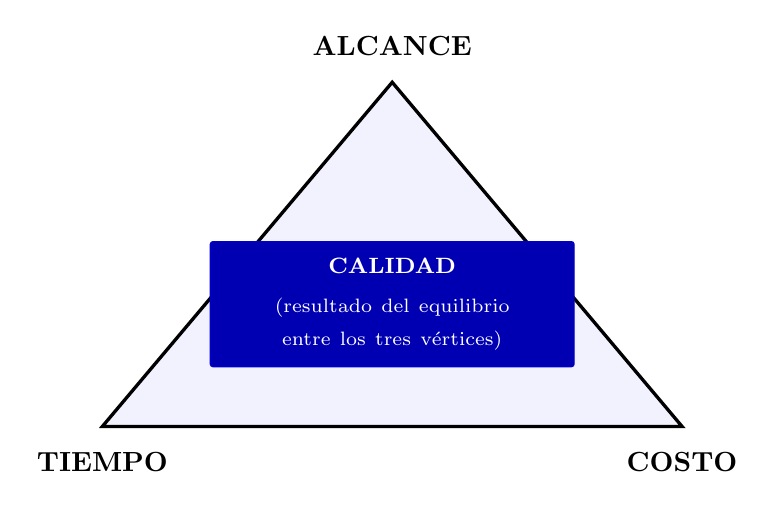
\begin{tikzpicture}[scale=1.15]
    \coordinate (Alcance) at (0, 3.8);
    \coordinate (Tiempo) at (-3.2, 0);
    \coordinate (Costo) at (3.2, 0);
    \draw[line width=1.2pt, fill=blue!5] (Alcance) -- (Tiempo) -- (Costo) -- cycle;
    \node[above=6pt] at (Alcance) {\textbf{ALCANCE}};
    \node[below=6pt] at (Tiempo) {\textbf{TIEMPO}};
    \node[below=6pt] at (Costo) {\textbf{COSTO}};
    \node[draw=blue!80!black, fill=blue!70!black, text=white, align=center, inner sep=6pt, rounded corners=1pt, text width=4.2cm] at (0, 1.35) {
        \textbf{\footnotesize CALIDAD}\\[2pt]
        \scriptsize (resultado del equilibrio entre los tres vértices)
    };
\end{tikzpicture}
\caption{Triángulo de restricciones y trade-offs del proyecto PyReach}
\label{fig:triangulo_restricciones}
\vspace{2pt}
\begin{flushleft}
\scriptsize \textit{Nota.} Esquema conceptual adaptado a la dinámica del proyecto según la Unidad 13 del libro de cátedra \parencite{pmi2021pmbok, torres2026proyecto}. Elaboración propia. %[cite: 1, 7]
\end{flushleft}
\end{figure}

En la Tabla \ref{tab:registro_tradeoffs} se documenta el registro formal de \textit{trade-offs} aceptados, conforme a la estructura de la Tabla 18 del modelo institucional y la Unidad 13 del libro de cátedra \parencite{torres2026proyecto}. %[cite: 1, 7]

\begin{table}[H]
\centering
\caption{Registro de trade-offs aceptados}
\label{tab:registro_tradeoffs}
\small
\setstretch{1.05}
\begin{tabularx}{\textwidth}{>{\raggedright\arraybackslash}p{3.5cm} >{\centering\arraybackslash}p{2.2cm} >{\centering\arraybackslash}p{2.2cm} >{\raggedright\arraybackslash}X}
\toprule
\textbf{Tensión identificada} & \textbf{Variable protegida} & \textbf{Variable ajustada} & \textbf{Justificación} \\
\midrule
Alcance vs. Tiempo & \textbf{Tiempo} & Alcance & 
El ciclo académico impone un límite estricto de 8 semanas efectivas (4 sprints quincenales) para la Fase 2 \parencite{torres2026proyecto}. %[cite: 2, 7]
Se restringe el análisis al plano estático (AST) y se adopta una heurística conservadora (\textit{Potencialmente alcanzable}) ante patrones dinámicos complejos \parencite{salis2021pycg}. \\ %[cite: 2, 4]
\addlinespace
Alcance vs. Costo & \textbf{Costo} & Alcance & 
El presupuesto disponible está restringido a un máximo de S/ 3,500.00 \parencite{torres2026proyecto}. %[cite: 2, 7]
Se excluye la generación automática de parches de código (\textit{auto-remediation}) para evitar tarifas recurrentes de modelos generativos comerciales de terceros \parencite{bogart2016break}. \\ %[cite: 2, 4]
\addlinespace
Tiempo vs. Costo y Calidad & \textbf{Tiempo y Calidad} & Alcance de construcción propia & 
Para no duplicar horas-hombre de desarrollo ni comprometer el cronograma, se reutilizan y adaptan librerías académicas consolidadas (\textit{NetworkX} y esquemas de \textit{PyCG}) en lugar de programar un motor de grafos desde cero \parencite{hagberg2008exploring, salis2021pycg}. \\ %[cite: 2, 4]
\bottomrule
\end{tabularx}
\vspace{2pt}
\begin{flushleft}
\scriptsize \textit{Nota.} Registro de decisiones de compensación ante la triple restricción formulado según la Unidad 13 del libro de cátedra \parencite{torres2026proyecto}. Elaboración propia. %[cite: 1, 7]
\end{flushleft}
\end{table}

\paragraph{Impacto de los trade-offs en los Requerimientos No Funcionales.}
Las decisiones de compensación adoptadas ejercen un impacto directo y controlado sobre la calidad:
\begin{itemize}[leftmargin=1.27cm]
    \item \textbf{Impacto en la Confidencialidad y Soberanía de Código (RNF-01):} Altamente positivo. Descartar servicios en la nube para análisis dinámico o remediación asegura la arquitectura 100\% local ($0\text{ bytes}$ en nube), cumpliendo el Control A.8.12 de ISO/IEC 27001:2022 \parencite{ladisa2023sok}. %[cite: 2, 4]
    \item \textbf{Impacto en la Precisión Analítica (RNF-02):} Controlado. La sobre-aproximación preventiva de llamadas dinámicas ambiguas evita omitir rutas inseguras (cero falsos negativos críticos), asegurando una reducción de alertas espurias $\ge 70\%$ en código estándar \parencite{pashchenko2022vuln4real, nielson1999principles}. %[cite: 2, 4]
    \item \textbf{Impacto en el Rendimiento en CI/CD (RNF-03):} Muy favorable. Al omitir la instrumentación en tiempo de ejecución y utilizar algoritmos de caminos optimizados con \textit{NetworkX}, el escaneo se mantiene por debajo de los 45 segundos por repositorio \parencite{hagberg2008exploring}. %[cite: 2, 4]
\end{itemize}

\paragraph{Declaración de la variable innegociable del proyecto.}
El equipo declara formalmente la jerarquía de gobierno ante contingencias durante la Fase 2 \parencite{torres2026proyecto}: %[cite: 2, 7]
\begin{enumerate}[leftmargin=1.27cm, label=\arabic*.]
    \item \textbf{Variable Innegociable: TIEMPO.} El cronograma académico impone una ventana fija de \textbf{8 semanas efectivas (4 sprints quincenales)} de desarrollo que no admite postergación \parencite{torres2026proyecto}. %[cite: 2, 7]
    \item \textbf{Variable Restringida: COSTO.} El presupuesto está topado en un techo máximo de S/ 3,500.00 financiado con recursos propios de los tesistas y herramientas libres de código abierto \parencite{torres2026proyecto}. %[cite: 2, 7]
    \item \textbf{Variable Negociable: ALCANCE.} Es la variable de ajuste primario. Ante cualquier retraso en un sprint superior al 15\% del esfuerzo planificado, se protegerá el tiempo recortando funcionalidades no esenciales (por ejemplo, postergar el parseo de archivos \texttt{Pipfile.lock} y priorizar exclusivamente \texttt{requirements.txt}), sin degradar la cobertura de pruebas bajo TDD ni la soberanía local de los datos \parencite{wiegers2013software, torres2026proyecto}. %[cite: 2, 7]
\end{enumerate}

% -------------------------------------------------------------------------
% 1.15. GESTIÓN DEL PROYECTO: CRONOGRAMA, TIEMPO Y COSTOS
% -------------------------------------------------------------------------
\subsection{Gestión del Proyecto: Cronograma, Tiempo y Costos}
Esta sección formaliza el plan de gestión del proyecto conforme a las directrices de la Unidad 14 del libro de cátedra \parencite{torres2026proyecto} y los estándares del PMBOK \parencite{pmi2021pmbok}, articulando el organigrama de gobierno, la Estructura de Descomposición del Trabajo (EDT), el cronograma detallado de actividades, el presupuesto paramétrico integral, la matriz inicial de riesgos y la cuantificación de las reservas de contingencia y costos de calidad \parencite{pressman2020software, torres2026proyecto}. %[cite: 1, 2, 7]

\subsubsection{Organigrama del Proyecto}
La estructura organizativa del proyecto se adapta a un equipo ágil de desarrollo en convenio técnico con Lidercom Perú S.A.C., prescindiendo de dependencias burocráticas intermedias (sin oficina de PMO) y unificando la ejecución técnica directamente en los dos tesistas \parencite{torres2026proyecto}. %[cite: 2, 7]
En la Figura \ref{fig:organigrama_gobierno} se presenta el organigrama general de gobierno y articulación operativa del proyecto \textit{PyReach}. %[cite: 1, 2]

\begin{figure}[H]
\centering
\includegraphics[width=0.68\textwidth]{figuras4/mermaid-diagram-2026-09-08-105837.png}
\caption{Organigrama general de gobierno y articulación operativa del proyecto PyReach}
\label{fig:organigrama_gobierno}
\vspace{2pt}
\begin{flushleft}
\scriptsize \textit{Nota.} Diagrama jerárquico de gobierno adaptado a la dinámica del proyecto capstone según la Unidad 14 del libro de cátedra \parencite{torres2026proyecto}. Elaboración propia. %[cite: 1, 2, 7]
\end{flushleft}
\end{figure}

En la Tabla \ref{tab:roles_responsabilidades} se especifican los roles, integrantes asignados, funciones primarias y líneas de reporte del equipo. 

\begin{table}[H]
\centering
\caption{Roles y responsabilidades del equipo de proyecto}
\label{tab:roles_responsabilidades}
\small
\setstretch{1.05}
\begin{tabularx}{\textwidth}{>{\bfseries\raggedright\arraybackslash}p{3.2cm} >{\raggedright\arraybackslash}p{3.4cm} X >{\raggedright\arraybackslash}p{2.6cm}}
\toprule
\textbf{Rol} & \textbf{Responsable (nombre)} & \textbf{Funciones principales} & \textbf{Reporta a} \\
\midrule
Sponsor / Asesor & 
Dr. Néstor Torres Gamarra & 
Supervisa la rigurosidad metodológica, autoriza el alcance técnico formal, aprueba las solicitudes de cambio y valida los cierres de fase \parencite{torres2026proyecto}. & 
Comité Académico UCSM \\ %[cite: 1, 2, 7]
\addlinespace
Jefe de Proyecto & 
Julio Centeno León y \newline José Alonso Yáñez Mejía & 
Co-Project Managers. Gestionan el backlog de sprint, monitorean el cronograma, administran el presupuesto de inversión y gestionan riesgos \parencite{pmi2021pmbok}. & 
Sponsor / Asesor \\ %[cite: 1, 2, 7]
\addlinespace
Analista / Diseñador & 
Julio Centeno León & 
Elicitación de requerimientos, diseño del motor sintáctico AST, resolución de tablas de símbolos y modelado de datos en SQLite \parencite{salis2021pycg}. & 
Jefe de Proyecto \\ %[cite: 1, 2]
\addlinespace
Desarrollador(a) & 
José Alonso Yáñez Mejía & 
Modelado del Grafo de Llamadas con \textit{NetworkX}, implementación del algoritmo de alcanzabilidad y serialización OASIS SARIF v2.1.0 \parencite{oasis2019sarif}. & 
Jefe de Proyecto \\ %[cite: 1, 2]
\addlinespace
Encargado(a) de Calidad y Pruebas & 
Luis Espinoza y \newline Andry Cáceres (Lidercom) & 
Usuarios Clave. Validan heurísticas sobre microservicios, supervisan pruebas unitarias TDD con \textit{pytest} y auditan la soberanía ISO 27001 \parencite{ladisa2023sok}. & 
Jefe de Proyecto \\ %[cite: 1, 2]
\bottomrule
\end{tabularx}
\vspace{2pt}
\begin{flushleft}
\scriptsize \textit{Nota.} Definición de funciones y líneas de reporte estructuradas según la Unidad 14 del libro de cátedra \parencite{torres2026proyecto}. Elaboración propia. %[cite: 1, 7]
\end{flushleft}
\end{table}

\subsubsection{Estructura de Descomposición del Trabajo (EDT)}
La Estructura de Descomposición del Trabajo (EDT/WBS) organiza el esfuerzo del proyecto en paquetes de trabajo jerárquicos y entregables verificables orientados al producto, aplicando la regla del 100\% del PMBOK \parencite{pmi2021pmbok, torres2026proyecto}. %[cite: 1, 2, 7]
En la Figura \ref{fig:fases_macro_proyecto} se ilustra la descomposición en las tres fases del curso (16 semanas en total). %[cite: 1, 2]

\begin{figure}[H]
\centering
\includegraphics[width=0.88\textwidth]{../figuras/figuras1/mermaid-diagram-2026-08-17-223026.png}
\caption{Estructura macro de las tres fases del proyecto (16 semanas)}
\label{fig:fases_macro_proyecto}
\end{figure}

A nivel operativo, la EDT desagrega el esfuerzo en tres niveles jerárquicos: \textbf{Nivel 1} (fases del ciclo académico: Fase 1 --- Semanas 1 a 4, 120 HH; Fase 2 --- Semanas 5 a 12, 240 HH; Fase 3 --- Semanas 13 a 16, 120 HH), \textbf{Nivel 2} (entregables mayores: componentes modulares de software, paquetes de mitigación técnica y normativa, artefactos de verificación y documentación) y \textbf{Nivel 3} (paquetes de trabajo y actividades técnicas operativas con responsable y entregable verificable) \parencite{pmi2021pmbok}. %[cite: 2]

En la Tabla \ref{tab:edt_proyecto_pyreach} se presenta la primera parte de la EDT, correspondiente a la fase de análisis con la mitigación normativa ISO 27001 y los dos primeros sprints de desarrollo junto con sus paquetes de mitigación técnica.

\begin{table}[H]
\centering
\caption{Estructura de Descomposición del Trabajo (EDT) del proyecto PyReach (Parte 1)}
\label{tab:edt_proyecto_pyreach}
\footnotesize
\singlespacing
\setlength{\tabcolsep}{3.0pt}
\renewcommand{\arraystretch}{0.88}
\begin{tabularx}{\textwidth}{>{\bfseries\raggedright\arraybackslash}p{1.2cm} >{\raggedright\arraybackslash}p{3.8cm} >{\raggedright\arraybackslash}X >{\centering\arraybackslash}p{2.3cm} >{\centering\arraybackslash}p{1.6cm}}
\toprule
\textbf{Cód.} & \textbf{Entregable Mayor (Nivel 2)} & \textbf{Paquetes de Trabajo / Actividades Técnicas (Nivel 3)} & \textbf{Responsable} & \textbf{Período} \\
\midrule
\multicolumn{5}{l}{\textbf{1.0 FASE 1: INTRODUCCIÓN Y ANÁLISIS (Semanas 1 a 4 --- 120 HH)}} \\
\midrule
1.1 & Perfil del Proyecto y Diagnóstico & 1.1.1 Caracterización del problema en microservicios Lidercom \parencite{pashchenko2022vuln4real}. \newline 1.1.2 Formulación de objetivos, justificación y matriz de consistencia. & Julio Centeno & Semanas 1--2 \\
\addlinespace
1.2 & Especificación y Mitigación Normativa ISO 27001 & 1.2.1 Especificación formal de RF (RF-01 a RF-10) y RNF bajo ISO/IEC 25010. \newline 1.2.2 Modelado de casos de uso y definición de la arquitectura local. \newline 1.2.3 \textbf{(Mitigación M8)} Autoestudio de controles ISO/IEC 27001:2022 (A.8.8, A.8.12, A.8.28) y sesión de juicio de expertos con auditor. & Alonso Yáñez \newline \textit{(Apoyo: Julio)} & Semanas 2--3 \newline Semanas 3--4 \\
\addlinespace
1.3 & Análisis de Alternativas y Viabilidad & 1.3.1 Ponderación multicriterio de alternativas (Alt. C seleccionada). \newline 1.3.2 Evaluación de viabilidad técnica, económica y financiera ($I_0 = \text{S/ } 3,500.00$). & Equipo Conjunto & Semana 4 \\
\midrule
\multicolumn{5}{l}{\textbf{2.0 FASE 2: DESARROLLO E IMPLEMENTACIÓN DEL ARTEFACTO (Semanas 5 a 12 --- 240 HH)}} \\
\midrule
2.1 & \textbf{Sprint 1:} Ingesta de Dependencias y Base Local OSV & 2.1.1 Parser de manifiestos directos y de bloqueo (\texttt{requirements.txt}). \newline 2.1.2 Base de datos SQLite con volcado indexado de OpenSSF OSV \parencite{openssf2023osv}. \newline 2.1.3 \textbf{(Mitigación M6)} Construcción de 5 fixtures sintéticos y pruebas TDD \parencite{myers2011art}. & Julio Centeno \newline \textit{(Apoyo: Alonso)} & Semanas 5--6 \\
\addlinespace
2.2 & Mitigaciones Técnicas M1 y M5 & 2.2.1 \textbf{(Mitigación M1)} Autoestudio del árbol interno CPython 3.10+ y \texttt{ast.NodeVisitor} \parencite{salis2021pycg}. \newline 2.2.2 \textbf{(Mitigación M5)} Normalización de rangos de versión de OSV para consultas locales \textit{offline}. & Julio Centeno & Semanas 5--6 \\
\addlinespace
2.3 & \textbf{Sprint 2:} Motor Sintáctico de Inspección de Código & 2.3.1 Extractor AST para funciones, llamadas y tablas de símbolos locales. \newline 2.3.2 Resolvedor recursivo de importaciones y alias en \texttt{site-packages}. \newline 2.3.3 Pruebas unitarias de resolución sintáctica sobre paquetes externos. & Julio Centeno & Semanas 7--8 \\
\addlinespace
2.4 & Mitigación Técnica M2 & 2.4.1 \textbf{(Mitigación M2)} Prototipado e inspección de rutas físicas en \texttt{site-packages} con PyCG. & Julio Centeno & Semanas 7--8 \\
\bottomrule
\end{tabularx}
\end{table}%
\newpage
\begin{table}[H]
\centering
\ContinuedFloat
\caption{Estructura de Descomposición del Trabajo (EDT) del proyecto PyReach (Continuación)}
\footnotesize
\singlespacing
\setlength{\tabcolsep}{3.0pt}
\renewcommand{\arraystretch}{0.88}
\begin{tabularx}{\textwidth}{>{\bfseries\raggedright\arraybackslash}p{1.2cm} >{\raggedright\arraybackslash}p{3.8cm} >{\raggedright\arraybackslash}X >{\centering\arraybackslash}p{2.3cm} >{\centering\arraybackslash}p{1.6cm}}
\toprule
\textbf{Cód.} & \textbf{Entregable Mayor (Nivel 2)} & \textbf{Paquetes de Trabajo / Actividades Técnicas (Nivel 3)} & \textbf{Responsable} & \textbf{Período} \\
\midrule
\multicolumn{5}{l}{\textbf{2.0 FASE 2: DESARROLLO (Continuación: Sprints 3, 4 y Documentación)}} \\
\midrule
2.5 & \textbf{Sprint 3:} Motor de Grafos y Alcanzabilidad & 2.5.1 Construcción del Call Graph interprocedimental con NetworkX \parencite{hagberg2008exploring}. \newline 2.5.2 Algoritmo de búsqueda de rutas de ejecución hacia funciones con CVE \parencite{ryder1979constructing}. \newline 2.5.3 Heurística preventiva de seguridad para metaprogramación dinámica. & Alonso Yáñez & Semanas 9--10 \\
\addlinespace
2.6 & Mitigaciones Técnicas M3 y M7 & 2.6.1 \textbf{(Mitigación M3)} Adaptación de estructuras \texttt{DiGraph} y control de profundidad ($k=5$). \newline 2.6.2 \textbf{(Mitigación M7)} Configuración del runner local corporativo en servidor de Lidercom \parencite{humble2010continuous}. & Alonso Yáñez & Semanas 9--10 \\
\addlinespace
2.7 & \textbf{Sprint 4:} CLI, Serializador SARIF y CI/CD & 2.7.1 \textbf{(Mitigación M4)} Validación estricta con \texttt{jsonschema} y reporte SARIF v2.1.0 \parencite{oasis2019sarif}. \newline 2.7.2 Interfaz CLI con códigos de salida bloqueantes (\textit{exit codes}). \newline 2.7.3 Suite de pruebas de integración completa con cobertura $\ge 80\%$. & Alonso Yáñez \newline \textit{(Apoyo: Julio)} & Semanas 11--12 \\
\addlinespace
2.8 & Documentación Técnica y Auditoría de Seguridad & 2.8.1 Manual de arquitectura interna, diseño de módulos y diagramas. \newline 2.8.2 Manual de instalación, configuración y uso de la interfaz CLI \parencite{torres2026proyecto}. \newline 2.8.3 Validación final de lista de chequeo ISO/IEC 27001 (Control A.8.12). & Equipo Conjunto & Semanas 11--12 \\
\midrule
\multicolumn{5}{l}{\textbf{3.0 FASE 3: VALIDACIÓN EXPERIMENTAL Y PRESENTACIÓN (Semanas 13 a 16 --- 120 HH)}} \\
\midrule
3.1 & Experimentación en Entorno Real & 3.1.1 Despliegue en pipeline CI/CD sobre microservicios reales de Lidercom. \newline 3.1.2 Medición empírica de reducción de falsas alertas ($\ge 70\%$) y precisión. \newline 3.1.3 Medición del tiempo de procesamiento en hardware local (umbral RNF-03 $<45\text{ s}$). & Equipo Conjunto & Semanas 13--14 \\
\addlinespace
3.2 & Evaluación Cuantitativa de Métricas & 3.2.1 Consolidación de matrices de confusión, curvas de precisión y tiempos de cómputo. & Julio Centeno & Semanas 14--15 \\
\addlinespace
3.3 & Redacción del Informe Final (Tesis) & 3.3.1 Redacción del Informe Final de Ingeniería de Software (conclusiones y anexos). & Equipo Conjunto & Semanas 15--16 \\
\addlinespace
3.4 & Preparación y Sustentación Final & 3.4.1 Preparación de diapositivas y defensa técnica pública ante jurado evaluador. & Equipo Conjunto & Semana 16 \\
\bottomrule
\end{tabularx}
\end{table}

\subsubsection{Cronograma General}
El cronograma articula las dependencias lógicas de precedencia (Fin a Inicio --- FS) y los plazos requeridos para cada paquete de trabajo \parencite{pmi2021pmbok, torres2026proyecto}. %[cite: 1, 2, 7]
En la Tabla \ref{tab:cronograma_general} se lista la secuencia técnica de actividades según la Tabla 20 del modelo institucional \parencite{torres2026proyecto}. %[cite: 1, 7]

\begin{table}[H]
\centering
\caption{Cronograma general}
\label{tab:cronograma_general}
\small
\setstretch{1.05}
\begin{tabularx}{\textwidth}{>{\raggedright\arraybackslash}p{6.8cm} >{\centering\arraybackslash}p{2.2cm} >{\centering\arraybackslash}p{2.2cm} >{\raggedright\arraybackslash}X}
\toprule
\textbf{Actividad} & \textbf{Duración} & \textbf{Predecesora} & \textbf{Responsable} \\
\midrule
1.1 Definición del problema, justificación y perfil & 2 semanas & --- & Julio Centeno \\
1.2 Especificación de requerimientos y RNF & 1 semana & 1.1 & José Alonso Yáñez \\
1.3 Ponderación de alternativas y viabilidad & 1 semana & 1.2 & Equipo Conjunto \\
\midrule
2.1 Sprint 1: Parser dependencias e ingesta OSV & 2 semanas & 1.3 & Julio Centeno \\
2.2 Mitigación M1/M5: Autoestudio AST y SQLite & 1 semana & 1.3 & Julio Centeno \\
2.3 Sprint 2: Motor sintáctico AST y resolución alias & 2 semanas & 2.1, 2.2 & Julio Centeno \\
2.4 Mitigación M2: Inspección en \texttt{site-packages} & 1 semana & 2.1 & Julio Centeno \\
2.5 Sprint 3: Call Graph NetworkX y alcanzabilidad & 2 semanas & 2.3 & José Alonso Yáñez \\
2.6 Mitigación M3/M7: Adaptación de NetworkX y runner & 1 semana & 2.3 & José Alonso Yáñez \\
2.7 Sprint 4: Serializador SARIF v2.1.0, CLI y CI/CD & 2 semanas & 2.5, 2.6 & José Alonso Yáñez \\
2.8 Documentación técnica y manual de usuario CLI & 1 semana & 2.7 & Equipo Conjunto \\
\midrule
3.1 Evaluación experimental en microservicios Lidercom & 2 semanas & 2.7, 2.8 & Equipo Conjunto \\
3.2 Evaluación cuantitativa de reducción de alertas & 1 semana & 3.1 & Julio Centeno \\
3.3 Redacción del Informe Final de Ingeniería & 2 semanas & 3.1 & Equipo Conjunto \\
3.4 Preparación de diapositivas y sustentación final & 1 semana & 3.2, 3.3 & Equipo Conjunto \\
\bottomrule
\end{tabularx}
\vspace{2pt}
\begin{flushleft}
\scriptsize \textit{Nota.} Dependencias lógicas de precedencia calculadas según la Unidad 14 del libro de cátedra \parencite{torres2026proyecto}. Elaboración propia. %[cite: 1, 2, 7]
\end{flushleft}
\end{table}

\paragraph{Diagrama de Gantt del proyecto.}
En cumplimiento del formato reglamentario del libro de cátedra \parencite{torres2026proyecto}, se presenta la programación temporal estructurada en una matriz de cuadrícula completa dividida en dos bloques secuenciales para preservar una óptima legibilidad sin sobreposición de texto \parencite{torres2026proyecto}. %[cite: 2, 7]

En la Tabla \ref{tab:gantt_bloque1} se detalla la programación de la Fase 1 y la primera mitad de la Fase 2 (Semanas 1 a 8) \parencite{torres2026proyecto}. %[cite: 2, 7]

\begin{table}[H]
\centering
\caption{Diagrama de Gantt del proyecto PyReach — Parte 1 (Semanas 1 a 8)}
\label{tab:gantt_bloque1}
\footnotesize
\singlespacing
\setlength{\tabcolsep}{2.5pt}
\renewcommand{\arraystretch}{1.10}
\begin{tabularx}{\textwidth}{|X|*{8}{>{\centering\arraybackslash}p{0.62cm}|}}
\hline
\textbf{Elemento / Fase del Proyecto} & \textbf{S1} & \textbf{S2} & \textbf{S3} & \textbf{S4} & \textbf{S5} & \textbf{S6} & \textbf{S7} & \textbf{S8} \\
\hline
\multicolumn{9}{|l|}{\textbf{Fase 1: Introducción y Análisis (Semanas 1 a 4)}} \\
\hline
1.1 Definición del problema, justificación y perfil inicial & X & X & & & & & & \\
\hline
1.2 Especificación de requerimientos y mitigación ISO (M8) & & X & X & & & & & \\
\hline
1.3 Ponderación de alternativas, viabilidad y entrega Práctica 4 & & & & X & & & & \\
\hline
\multicolumn{9}{|l|}{\textbf{Fase 2: Desarrollo del Proyecto — Sprints 1 y 2 (Semanas 5 a 8)}} \\
\hline
2.1 Sprint 1: Parser dependencias, ingesta OSV y fixtures TDD & & & & & X & X & & \\
\hline
2.2 Mitigación M1/M5: Autoestudio AST e indexación SQLite \textit{offline} & & & & & X & & & \\
\hline
2.3 Sprint 2: Motor sintáctico AST y resolución de llamadas & & & & & & & X & X \\
\hline
2.4 Mitigación M2: Prototipado de inspección en \texttt{site-packages} & & & & & & & X & \\
\hline
\end{tabularx}
\vspace{2pt}
\begin{flushleft}
\scriptsize \textit{Nota.} Programación correspondiente a las primeras ocho semanas del semestre \parencite{torres2026proyecto}. Elaboración propia. %[cite: 2, 7]
\end{flushleft}
\end{table}

En la Tabla \ref{tab:gantt_bloque2} se detalla la programación de la segunda mitad de la Fase 2 y la Fase 3 (Semanas 9 a 16) \parencite{torres2026proyecto}. %[cite: 2, 7]

\begin{table}[H]
\centering
\caption{Diagrama de Gantt del proyecto PyReach — Parte 2 (Semanas 9 a 16)}
\label{tab:gantt_bloque2}
\footnotesize
\singlespacing
\setlength{\tabcolsep}{2.5pt}
\renewcommand{\arraystretch}{1.10}
\begin{tabularx}{\textwidth}{|X|*{8}{>{\centering\arraybackslash}p{0.62cm}|}}
\hline
\textbf{Elemento / Fase del Proyecto} & \textbf{S9} & \textbf{S10} & \textbf{S11} & \textbf{S12} & \textbf{S13} & \textbf{S14} & \textbf{S15} & \textbf{S16} \\
\hline
\multicolumn{9}{|l|}{\textbf{Fase 2: Desarrollo del Proyecto — Sprints 3 y 4 (Semanas 9 a 12)}} \\
\hline
2.5 Sprint 3: Call Graph interprocedimental y alcanzabilidad & X & X & & & & & & \\
\hline
2.6 Mitigación M3/M7: Adaptación de NetworkX y runner local CI/CD & X & & & & & & & \\
\hline
2.7 Sprint 4: Serializador SARIF v2.1.0, CLI y compuertas CI/CD & & & X & X & & & & \\
\hline
2.8 Documentación técnica de software y auditoría ISO 27001 & & & & X & & & & \\
\hline
\multicolumn{9}{|l|}{\textbf{Fase 3: Validación Experimental y Cierre (Semanas 13 a 16)}} \\
\hline
3.1 Evaluación experimental sobre microservicios reales en Lidercom & & & & & X & X & & \\
\hline
3.2 Evaluación cuantitativa de reducción de falsos positivos ($\ge 70\%$) & & & & & & X & X & \\
\hline
3.3 Redacción del Informe Final de Ingeniería de Software (tesis) & & & & & & & X & X \\
\hline
3.4 Preparación de material de exposición y sustentación final & & & & & & & & X \\
\hline
\end{tabularx}
\vspace{2pt}
\begin{flushleft}
\scriptsize \textit{Nota.} Programación de cierre de desarrollo y fase de validación experimental \parencite{torres2026proyecto}. Elaboración propia. %[cite: 2, 7]
\end{flushleft}
\end{table}

\subsubsection{Cálculo Paramétrico de Costos}
Siguiendo la técnica de estimación paramétrica del PMBOK \parencite{pmi2021pmbok}, el costo directo de cada paquete de trabajo de la EDT se cuantifica multiplicando el esfuerzo en horas-hombre asignado por la tarifa horaria de subvención preprofesional de décimo semestre en Arequipa (\textbf{S/ 12.50 por hora-hombre}) \parencite{torres2026proyecto}. %[cite: 1, 2, 7]
En la Tabla \ref{tab:costos_parametricos_edt} se desglosa el cálculo paramétrico por actividad, en cumplimiento de la Tabla 21 del modelo institucional \parencite{torres2026proyecto}. %[cite: 1, 7]

\begin{table}[H]
\centering
\caption{Cálculo paramétrico de costos por actividad de la EDT}
\label{tab:costos_parametricos_edt}
\small
\setstretch{1.05}
\setlength{\tabcolsep}{4.5pt} % Optimiza el espacio entre columnas
\begin{tabularx}{\textwidth}{>{\raggedright\arraybackslash}X >{\raggedright\arraybackslash}p{3.8cm} c c r r}
\toprule
\textbf{Actividad (EDT)} & \textbf{Recurso asignado} & \textbf{Cant.} & \textbf{Unidad} & \textbf{Costo unit. (S/)} & \textbf{Costo total (S/)} \\
\midrule
2.1 Sprint 1: Ingesta OSV y Parser & Tesista (Julio Centeno) & 40 & Horas & S/ 12.50 & S/ 500.00 \\
2.3 Sprint 2: Motor sintáctico AST & Tesista (Julio Centeno) & 40 & Horas & S/ 12.50 & S/ 500.00 \\
2.5 Sprint 3: Call Graph y alcanzabilidad & Tesista (Alonso Yáñez) & 40 & Horas & S/ 12.50 & S/ 500.00 \\
2.7 Sprint 4: Módulo SARIF, CLI y CI/CD & Tesista (Alonso Yáñez) & 40 & Horas & S/ 12.50 & S/ 500.00 \\
2.2/2.4/2.6 Mitigación de brechas técnicas (M1--M7) & Equipo (Julio y Alonso) & 40 & Horas & S/ 12.50 & S/ 500.00 \\
2.8 Documentación técnica y auditoría ISO 27001 & Equipo (Julio y Alonso) & 40 & Horas & S/ 12.50 & S/ 500.00 \\
\midrule
\multicolumn{5}{l}{\textbf{Subtotal Paramétrico Base de Recursos Humanos}} & \textbf{S/ 3,000.00} \\
\bottomrule
\end{tabularx}
\vspace{2pt}
\begin{flushleft}
\scriptsize \textit{Nota.} Estimación paramétrica de esfuerzo integral ($240\text{ HH} \times \text{S/ } 12.50\text{/HH} = \text{S/ } 3,000.00$), que integra el desarrollo directo de los cuatro sprints (160 HH), las acciones de mitigación de brechas (40 HH) y la documentación técnica con auditoría normativa (40 HH), formulada según la Unidad 14 del libro de cátedra \parencite{torres2026proyecto}. Elaboración propia.
\end{flushleft}
\end{table}

\subsubsection{Matriz de Riesgos Inicial}
En cumplimiento estricto de la Tabla 22 del modelo institucional y de la Tabla 31 de la Unidad 14 del libro de cátedra \parencite{torres2026proyecto}, se identificaron ocho riesgos analizados en tres categorías: \textbf{técnicos, de negocio y de gestión}, asignando a cada uno su nivel de probabilidad, impacto y plan de respuesta concreto \parencite{pmi2021pmbok, torres2026proyecto}. %[cite: 1, 2, 7]
En la Tabla \ref{tab:matriz_riesgos_inicial} se detalla la matriz de riesgos inicial del proyecto. %[cite: 1, 2]

% ==========================================
% PARTE 1: Riesgos Técnicos (R1 a R4)
% ==========================================
\begin{table}[H]
\centering
\caption{Matriz de riesgos inicial (Parte 1: Riesgos técnicos)}
\label{tab:matriz_riesgos_inicial}
\small
\setstretch{1.05}
\begin{tabularx}{\textwidth}{>{\raggedright\arraybackslash}p{4.4cm} >{\centering\arraybackslash}p{2.0cm} >{\centering\arraybackslash}p{2.3cm} >{\centering\arraybackslash}p{1.8cm} X}
\toprule
\textbf{Riesgo} & \textbf{Categoría} & \textbf{Probabilidad} & \textbf{Impacto} & \textbf{Mitigación} \\
\midrule
R1. Explosión combinatoria en el grafo por dependencias densamente acopladas & 
Técnico & 
Media (20\%) & 
Alto & 
Limitar la profundidad máxima de búsqueda a $k=5$ saltos y emplear estructuras \texttt{DiGraph} de NetworkX optimizadas en memoria \parencite{hagberg2008exploring}. \\
\addlinespace
R2. Falsos negativos causados por metaprogramación dinámica en Python & 
Técnico & 
Media (25\%) & 
Medio & 
Implementar una heurística preventiva que clasifique llamadas no deterministas como \textit{Potencialmente alcanzables} \parencite{salis2021pycg}. \\
\addlinespace
R3. Rechazo del reporte por inconsistencias contra el esquema SARIF v2.1.0 & 
Técnico & 
Baja (10\%) & 
Alto & 
Validar automáticamente la estructura JSON de salida con la librería \texttt{jsonschema} contra el esquema formal en pruebas TDD \parencite{oasis2019sarif}. \\
\addlinespace
R4. No conformidad o fuga accidental de código frente a controles ISO/IEC 27001:2022 & 
Técnico & 
Baja (10\%) & 
Alto & 
Auditar mediante lista de verificación con el experto externo y validar estrictamente el aislamiento de red en el runner local (Control A.8.12) \parencite{gutierrez2024auditoria}. \\
\bottomrule
\end{tabularx}
\vspace{2pt}
\begin{flushleft}
\scriptsize \textit{Nota.} Clasificación integral de amenazas según la Unidad 14 del libro de cátedra \parencite{torres2026proyecto}. Continúa en la siguiente página.
\end{flushleft}
\end{table}

% ==========================================
% PARTE 2: Riesgos de Negocio y Gestión (R5 a R8)
% ==========================================
\begin{table}[H]
\centering
\ContinuedFloat % Mantiene el mismo número de tabla
\caption{Matriz de riesgos inicial (Parte 2: Riesgos de negocio y gestión)}
\small
\setstretch{1.05}
\begin{tabularx}{\textwidth}{>{\raggedright\arraybackslash}p{4.4cm} >{\centering\arraybackslash}p{2.0cm} >{\centering\arraybackslash}p{2.3cm} >{\centering\arraybackslash}p{1.8cm} X}
\toprule
\textbf{Riesgo} & \textbf{Categoría} & \textbf{Probabilidad} & \textbf{Impacto} & \textbf{Mitigación} \\
\midrule
R5. Demora en el acceso a microservicios y código real de Lidercom & 
Negocio & 
Media (20\%) & 
Alto & 
Coordinar accesos con dos semanas de anticipación y disponer de un repositorio réplica contenerizado en Docker como contingencia \parencite{humble2010continuous}. \\
\addlinespace
R6. Indisponibilidad temporal o rotación del contacto técnico en Lidercom & 
Negocio & 
Baja (10\%) & 
Alto & 
Elaborar manuales operativos autosuficientes (paquete 2.8) y acordar canales de validación asíncronos vía \textit{Pull Requests} con la gerencia \parencite{torres2026proyecto}. \\
\addlinespace
R7. Sobrecarga académica durante exámenes parciales de la universidad & 
Gestión & 
Alta (30\%) & 
Medio & 
Asignar un colchón (\textit{buffer}) de 3 días por sprint y programar las tareas pesadas fuera de las semanas 8 y 16 \parencite{pmi2021pmbok}. \\
\addlinespace
R8. Desviación temporal por subestimación en la complejidad del AST & 
Gestión & 
Media (10\%) & 
Alto & 
Aplicar el criterio innegociable: recortar el soporte de manifiestos secundarios (postergar \texttt{Pipfile.lock}) protegiendo el tiempo \parencite{torres2026proyecto}. \\
\bottomrule
\end{tabularx}
\vspace{2pt}
\begin{flushleft}
\scriptsize \textit{Nota.} Clasificación integral de amenazas según la Unidad 14 del libro de cátedra \parencite{torres2026proyecto}. Elaboración propia.
\end{flushleft}
\end{table}

\paragraph{Costo de Riesgos — Reserva de Contingencia (EMV).}
Para fundamentar cuantitativamente la reserva de contingencia sin recurrir a asignaciones arbitrarias, se toma cada riesgo identificado en la matriz de riesgos (Tabla \ref{tab:matriz_riesgos_inicial}), se le asigna su probabilidad porcentual y su impacto económico estimado en moneda nacional, calculando el Valor Monetario Esperado mediante la ecuación $\text{EMV} = \text{Probabilidad} \times \text{Impacto}$ \parencite{pmi2021pmbok, torres2026proyecto}. %[cite: 1, 7]
En la Tabla \ref{tab:reserva_emv} se desglosa el cálculo conforme a la Tabla 24 del modelo institucional \parencite{torres2026proyecto}. %[cite: 1, 7]

\begin{table}[H]
\centering
\caption{Costo de riesgos — reserva de contingencia (EMV)}
\label{tab:reserva_emv}
\small
\setstretch{1.05}
\begin{tabularx}{\textwidth}{>{\raggedright\arraybackslash}p{6.4cm} >{\centering\arraybackslash}p{2.2cm} >{\centering\arraybackslash}p{2.6cm} >{\raggedleft\arraybackslash}X}
\toprule
\textbf{Riesgo (de 1.15.5)} & \textbf{Probabilidad (\%)} & \textbf{Impacto económico (S/)} & \textbf{Valor Monetario Esperado — EMV (S/)} \\
\midrule
R1. Explosión combinatoria en grafos NetworkX & 20 \% & S/ 300.00 & S/ 60.00 \\
R2. Constructos dinámicos en Python & 25 \% & S/ 200.00 & S/ 50.00 \\
R3. Inconsistencias con esquema SARIF v2.1.0 & 10 \% & S/ 400.00 & S/ 40.00 \\
R4. No conformidad o fuga de código frente a ISO 27001 & 10 \% & S/ 300.00 & S/ 30.00 \\
R5. Demora en acceso a microservicios Lidercom & 20 \% & S/ 250.00 & S/ 50.00 \\
R6. Rotación del contacto técnico en Lidercom & 10 \% & S/ 200.00 & S/ 20.00 \\
R7. Sobrecarga académica en exámenes parciales & 30 \% & S/ 100.00 & S/ 30.00 \\
R8. Desviación temporal en complejidad de AST & 10 \% & S/ 200.00 & S/ 20.00 \\
\midrule
\multicolumn{3}{l}{\textbf{Reserva de contingencia por riesgos ($\sum\text{EMV}$)}} & \textbf{S/ 300.00} \\
\bottomrule
\end{tabularx}
\vspace{2pt}
\begin{flushleft}
\scriptsize \textit{Nota.} Cuantificación analítica de la reserva contingente según el PMBOK y la Unidad 14 \parencite{pmi2021pmbok, torres2026proyecto}. Elaboración propia. %[cite: 1, 7]
\end{flushleft}
\end{table}

\subsubsection{Resumen General de Costos del Proyecto}
En cumplimiento de la Tabla 25 del modelo institucional y de las Unidades 12 y 14 del libro de cátedra \parencite{torres2026proyecto}, en la Tabla \ref{tab:resumen_general_costos} se consolida en una estructura unificada el costo paramétrico directo por recursos humanos, las partidas de soporte, los gastos de bolsillo de los tesistas, el costo de calidad (COQ) y la reserva de contingencia por riesgos (EMV) \parencite{pmi2021pmbok, torres2026proyecto}. %[cite: 1, 7]

\begin{table}[H]
\centering
\caption{Resumen general de costos del proyecto}
\label{tab:resumen_general_costos}
\small
\setstretch{1.05}
\begin{tabularx}{\textwidth}{>{\raggedright\arraybackslash}p{7.2cm} >{\raggedleft\arraybackslash}p{3.2cm} >{\raggedleft\arraybackslash}X}
\toprule
\textbf{Categoría de costo} & \textbf{Costo total (S/)} & \textbf{\% del presupuesto} \\
\midrule
Recursos humanos (240 HH del equipo, incluye COQ absorbido de S/ 600.00 --- paramétrico base de 1.15.4) & S/ 3,000.00 & 85.7 \% \\
Software y licencias (Stack Open Source: Python, Poetry, SQLite) & S/ 0.00 & 0.0 \% \\
Hardware y equipos (Estaciones personales y servidor local Lidercom) & S/ 0.00 & 0.0 \% \\
Servicios (Conectividad a internet y movilidad local compartida) & S/ 200.00 & 5.7 \% \\
Reserva de contingencia por riesgos ($\sum\text{EMV}$ de 1.15.6) & S/ 300.00 & 8.6 \% \\
\midrule
\textbf{Presupuesto total del proyecto} & \textbf{S/ 3,500.00} & \textbf{100.0 \%} \\
\bottomrule
\end{tabularx}
\vspace{2pt}
\begin{flushleft}
\scriptsize \textit{Nota.} Consolidación presupuestal integral del software según la Unidad 14 del libro de cátedra \parencite{torres2026proyecto}. Elaboración propia. %[cite: 1, 2, 7]
\end{flushleft}
\end{table}

\paragraph{Verificación de consistencia presupuestal.}
Se comprueba de manera estricta que el presupuesto total consolidado en la Tabla \ref{tab:resumen_general_costos} asciende a exactamente \textbf{S/ 3,500.00}, cifra que guarda una concordancia matemática del 100\% con el costo de inversión inicial ($I_0$) reportado en el análisis de recursos (1.13.1) y en el flujo de caja descontado de la evaluación económica y financiera (1.13.3), cerrando con consistencia la planificación integral del Perfil de Proyecto \parencite{torres2026proyecto}. %[cite: 1, 2, 7]